\chapter{Mô hình}

\section{Mô hình Dự đoán giá trong ngày sử dụng Định luật Bayes}
Ở chương 4, ta xét thấy sự tương quan tương đối lớn giữa hoạt động của người dùng diễn đàn FireAnt và diễn biến của thị trường, ta hãy cùng phân tích và áp dụng một số mô hình để kiểm chứng lại sự tương quan. Ở phần này, ta sẽ tập trung vào việc dự đoán sự tăng hoặc giảm của giá cổ phiếu dựa trên những bài viết trên diễn đàn FireAnt. Dưới đây là diễn giải của một mô hình xác suất thống kê sử dụng Định luật Bayes.

\subsection{Chuẩn bị dữ liệu tính toán}
 
\begin{center}
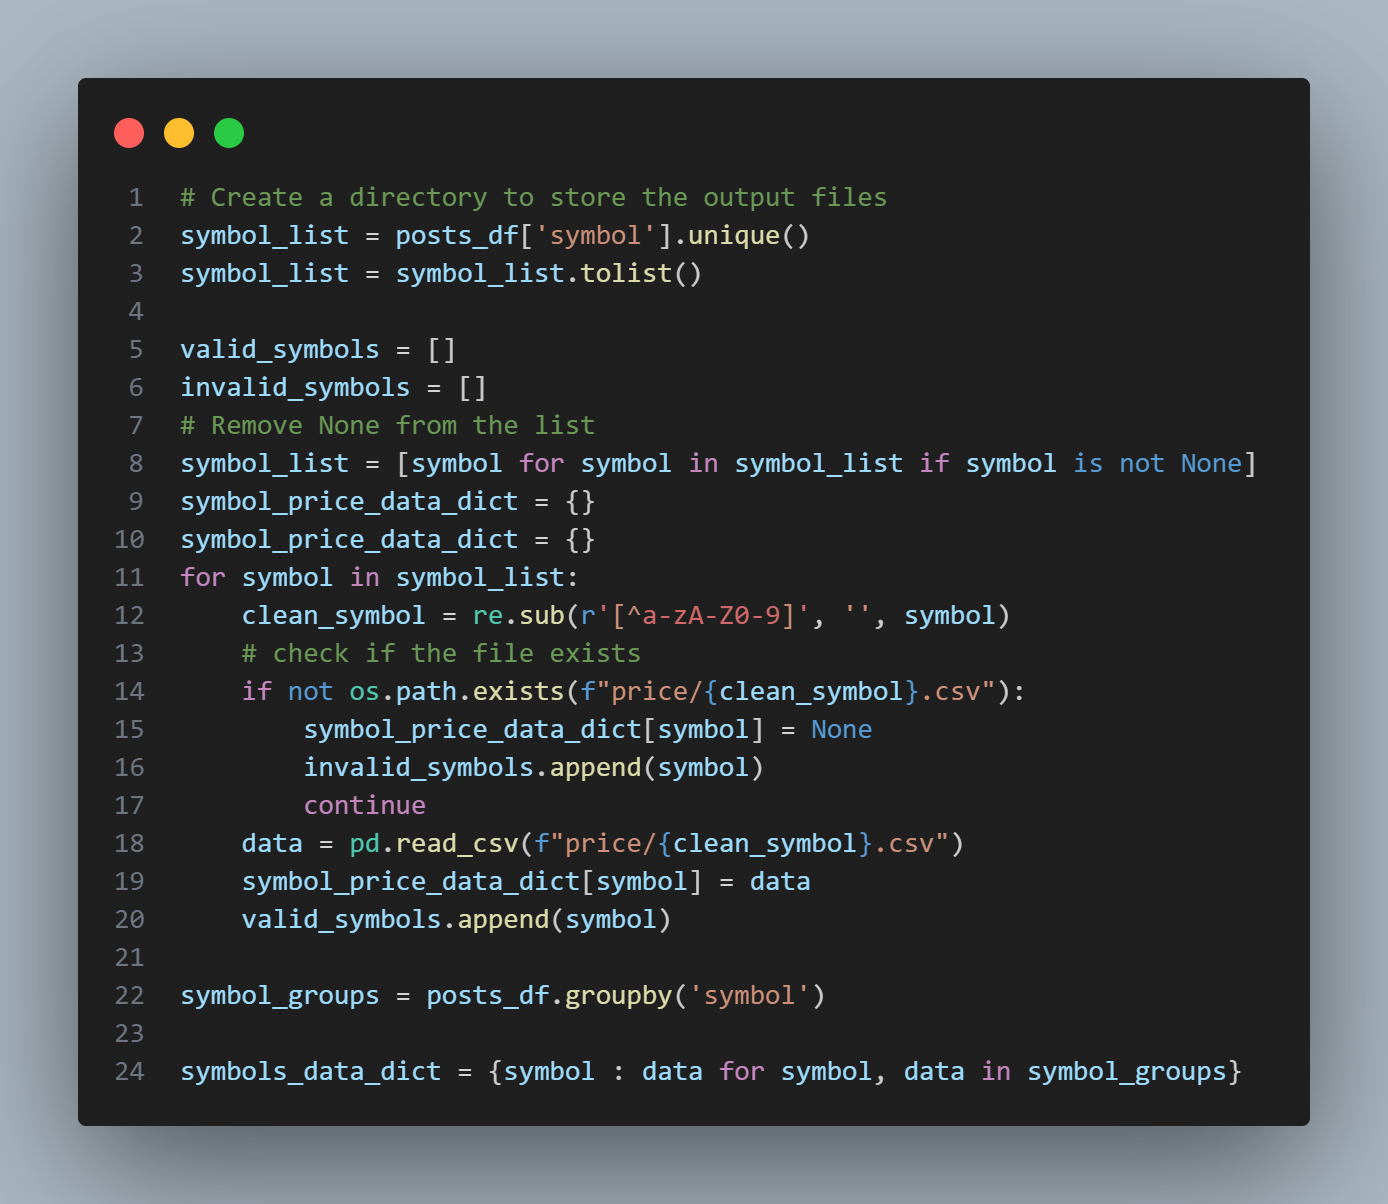
\includegraphics[width=0.75\linewidth]{images/code-5.1.png}
\end{center}

Ta lấy danh sách các mã chứng khoán từ file CSV \texttt{cleaned\_posts.csv} và đọc dữ liệu lịch sử giá của các mã đó vào \texttt{symbol\_price\_data\_dict}. Tiếp theo, ta chuẩn bị một dataframe gồm các chỉ số thống kê bài viết được nhóm theo ngày, bao gồm Số lượng bài viết; Số bài viết Tích cực; Số bài viết Tiêu cực; Số từ trung bình của bài viết; Tổng số lượt Thích; Tổng số lượt Bình luận.\\

Đồng thời kết hợp cùng dữ liệu giá cổ phiếu theo ngày, bao gồm Giá mở cửa; Giá cao nhất; Giá đóng cửa; Sự thay đổi giá trong ngày. Tất nhiên, ta chỉ lấy những ngày có diễn ra giao dịch.

\begin{center}
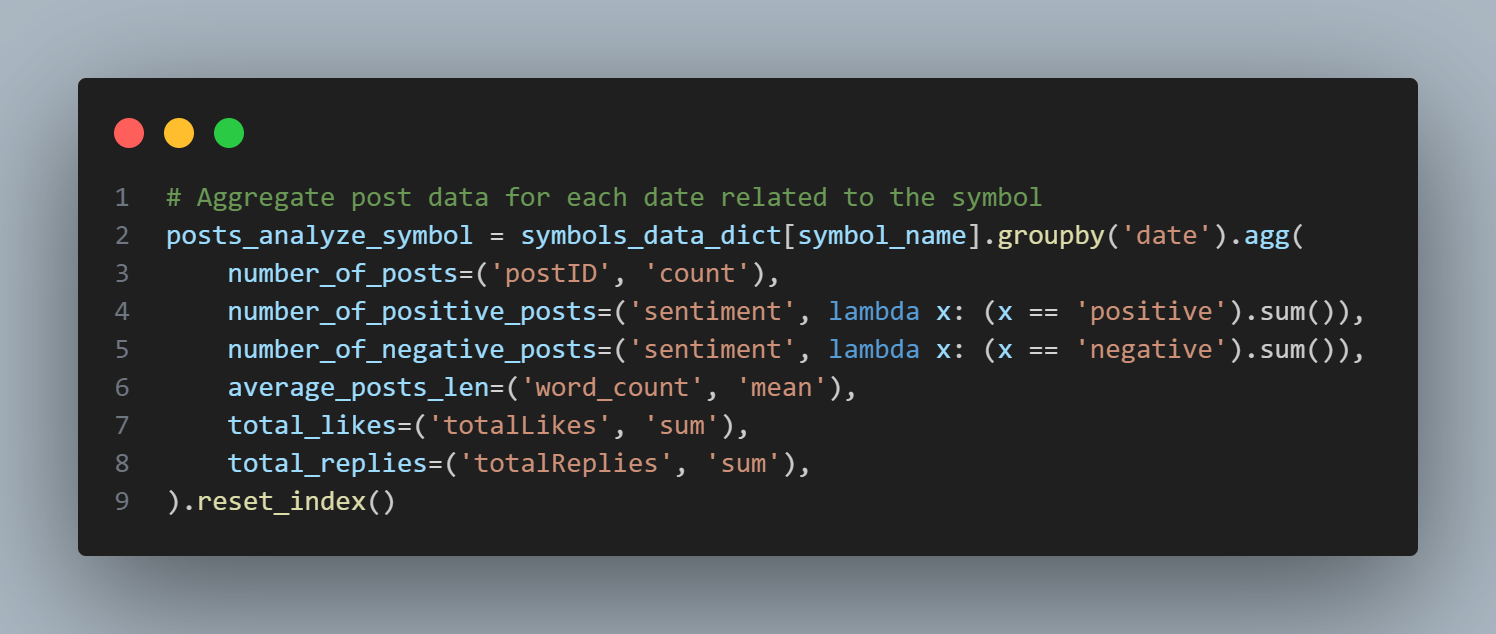
\includegraphics[width=0.8\linewidth]{images/code-5.2.png}
\end{center}

Kết quả là một dataframe mới với các cột:

\texttt{date, number\_of\_posts, number\_of\_positive\_posts, number\_of\_negative\_posts} 

\texttt{average\_posts\_len, total\_likes, total\_replies, open, high, close, daily\_change}.

\begin{center}
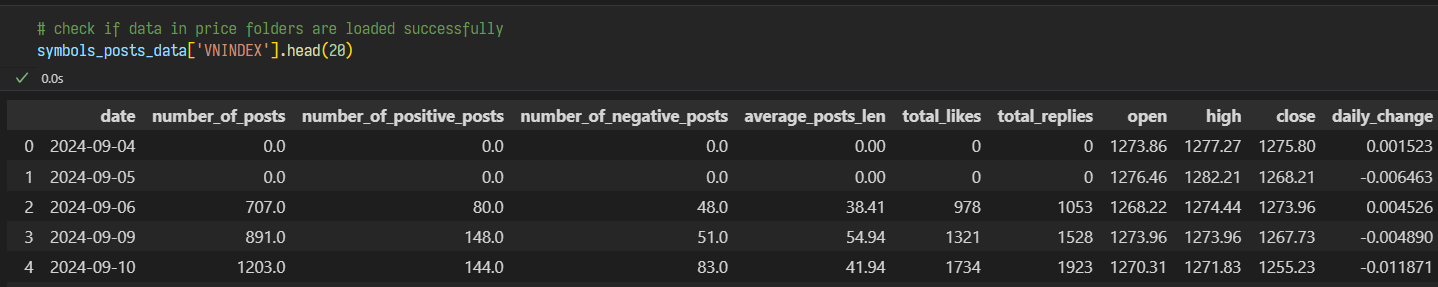
\includegraphics[width=1\linewidth]{images/code-5.3-aggreresult.png}
\end{center}

\subsection{Áp dụng Định luật Bayes}
Trước hết ta sẽ xây dựng hàm \texttt{bayesProbPosts} để thực hiện tính toán xác suất giá trị cổ phiếu thay đổi trong ngày. Dữ liệu trong hàm bao gồm ba cột: \texttt{date} (ngày giao dịch), \texttt{daily\_change} (phần trăm thay đổi giá cổ phiếu hàng ngày), và \texttt{number\_of\_posts} (số lượng bài viết trong ngày). Các cột này được kết hợp vào một dataframe duy nhất để dễ dàng xử lý và phân tích.\\

Tiếp theo ta xác định ngưỡng để phân định một ngày bất kỳ có số lượng bài viết là nhiều, ít, hay trung bình. Ta sẽ tính trung bình số lượng bài viết, sau đó phân định:
\begin{itemize}
\item Nếu số lượng bài viết ngày \textbf{lớn hơn 15\% mức trung bình}: Ngày này có lượng bài viết \textbf{nhiều};
\item Nếu số lượng bài viết trong ngày \textbf{nhỏ hơn 15\% mức trung bình}: Ngày này có lượng bài viết \textbf{ít};
\item Trường hợp còn lại: Ngày này có lượng bài viết \textbf{trung bình}.
\end{itemize}

Tương tự, với phần trăm thay đổi giá (\texttt{price\_column}):
\begin{itemize}
\item Nếu phần trăm thay đổi giá \textbf{lớn hơn 0.2\%}: Ngày này có giá \textbf{tăng};
\item Nếu phần trăm thay đổi giá \textbf{nhỏ hơn -0.2\%}: Ngày này có giá \textbf{giảm};
\item Trường hợp còn lại: Ngày này có giá \textbf{ít biến động}.
\end{itemize}

Như vậy, một ngày giao dịch có thể có \textbf{9 trường hợp kết quả xảy ra}. Với mỗi trường hợp, hàm \texttt{bayesProbPosts} sẽ tính ra giá trị xác suất cụ thể. Bằng cách sử dụng Định luật Bayes, giả sử với trường hợp (Giá tăng, Bài nhiều), ta có những xác suất sau:

 \[
P(\text{Giá tăng} \mid \text{Bài nhiều}) = \frac{P(\text{Bài nhiều} \mid \text{Giá tăng}) \times P(\text{Giá tăng})}{P(\text{Bài nhiều})}
\]

\[
P(\text{Bài nhiều} \mid \text{Giá tăng}) = \frac{P(\text{Số ngày Bài nhiều và Giá tăng})}{P(\text{Giá tăng})}
\]

\[
P(\text{Bài nhiều}) = \frac{\sum (\text{dataframe['Số bài trong ngày']} \geq \text{Ngưỡng xác định})}{\text{Số ngày giao dịch}}
\]

\[
P(\text{Giá tăng}) = \frac{\sum (\text{dataframe['Thay đổi giá trong ngày']} \geq \text{Ngưỡng xác định})}{\text{Số ngày giao dịch}}
\]

\begin{center}
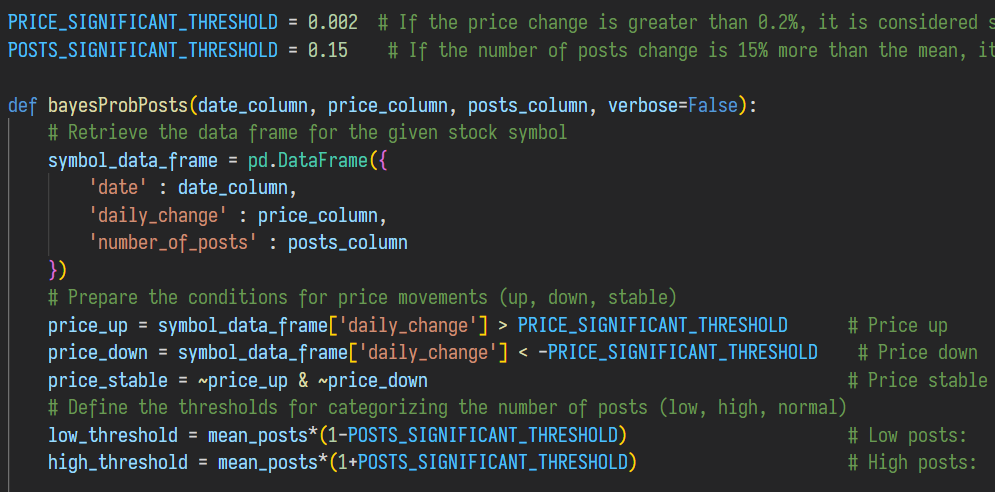
\includegraphics[width=0.7\linewidth]{images/code-5.4.png}
\end{center}

Ta tiến hành áp hàm này vào 3 yếu tố: Số bài viết trong ngày; Số bài viết Tích cực trong ngày; Số bài viết Tiêu cực trong ngày. Sau đó ta sẽ trực quan hóa kết quả bằng các biểu đồ Heatmap.

\begin{center}
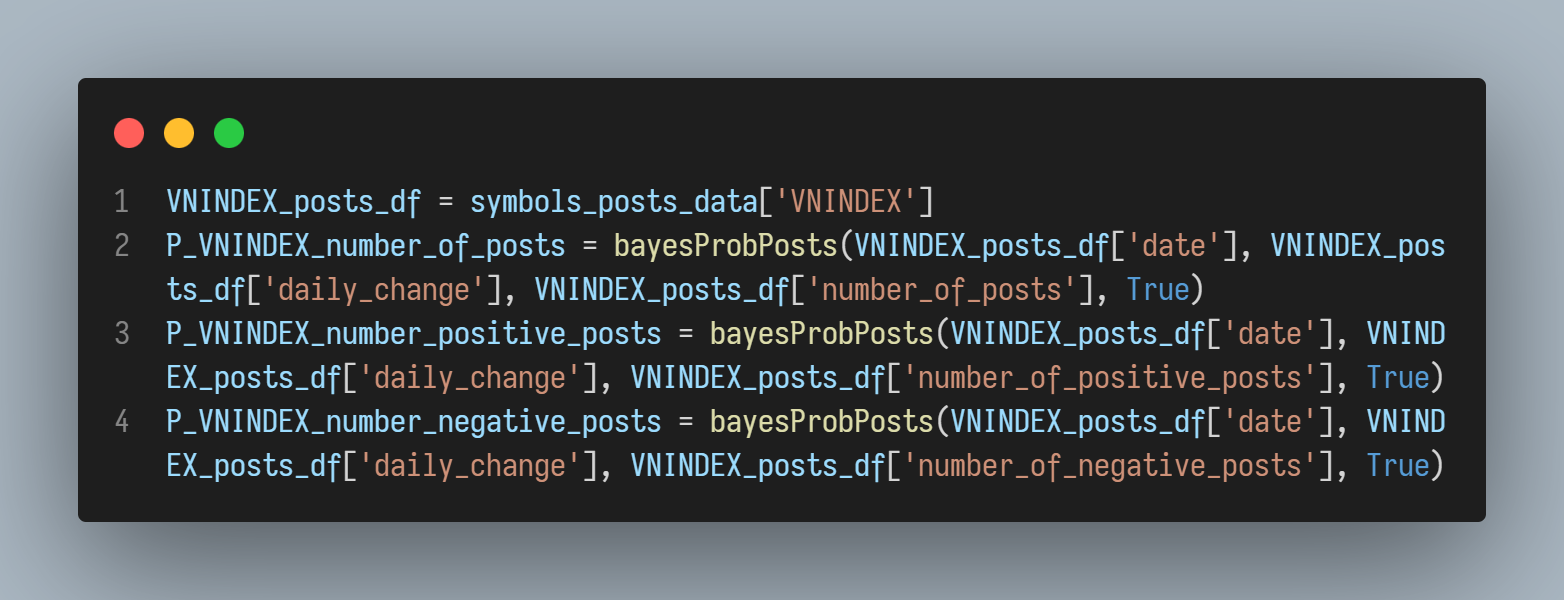
\includegraphics[width=0.75\linewidth]{images/code-5.5.png}
\end{center}

\subsection{Kiểm chứng Phương pháp}
\subsubsection*{Nhận xét Phương pháp trên VNINDEX}
 \begin{figure}[H]
     \centering
     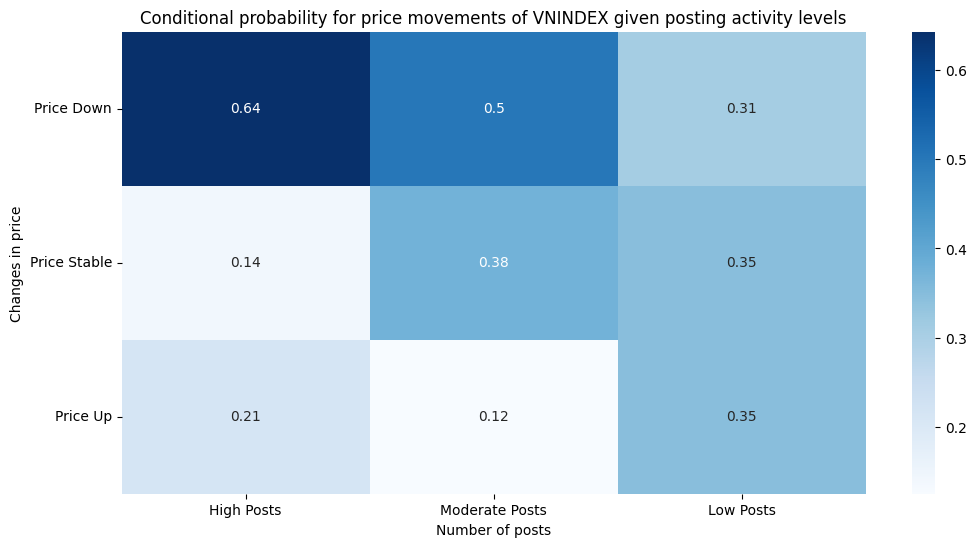
\includegraphics[width=0.9\linewidth]{images/plot-5.1-hmvniall.png}
     \caption{Heatmap Xác suất sự thay đổi của VNINDEX dựa trên Số bài đăng hàng ngày}
     \label{fig:5.1}
 \end{figure}

Ta sẽ đánh giá phương pháp này dựa trên kết quả của nó khi áp với giá trị của chỉ số VNINDEX. Với biểu đồ trên, ta có thể nhận xét khi có nhiều bài đăng trong ngày, thì VNINDEX sẽ có $64\%$ khả năng giảm giá. Khi lượng bài viết ở mức trung bình, xu hướng giảm giá vẫn tương đối rõ rệt, khi chỉ có $12\%$ xác suất giá sẽ tăng. Cuối cùng, khi có ít bài viết trong ngày, kết quả sẽ tương đối khó đoán định, có thể do đó là những ngày thị trường chán nản, thanh khoản thấp.

\begin{figure}[H]
    \centering
    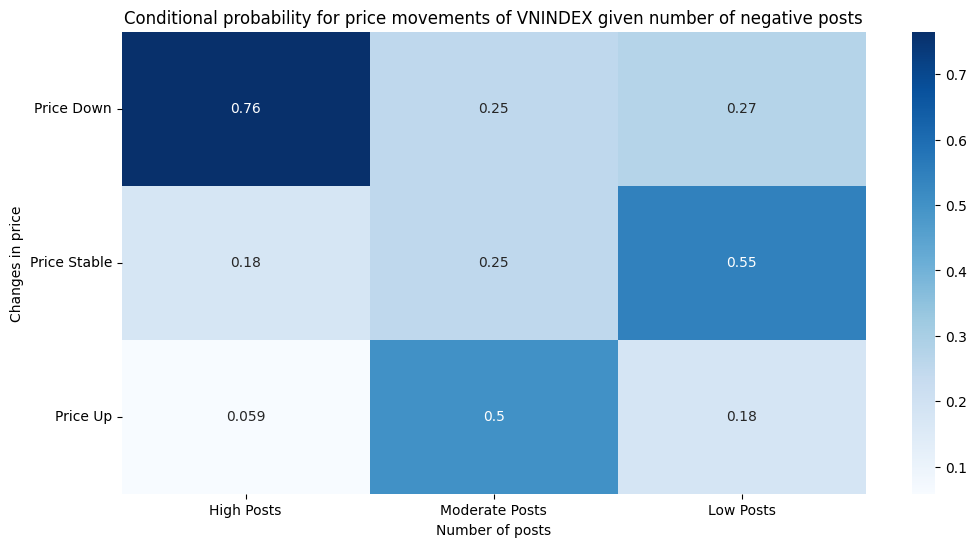
\includegraphics[width=0.9\linewidth]{images/plot-5.2-hmvnineg.png}
    \caption{Heatmap Xác suất sự thay đổi của VNINDEX dựa trên Số bài đăng Tiêu cực hàng ngày}
    \label{fig:5.2}
\end{figure}

Khi xét số lượng bài tiêu cực, ta dễ dàng nhận thấy khi có nhiều bài đăng tiêu cực trong ngày, thì VNINDEX sẽ có khả năng giảm giá cao. Tuy vậy, khi lượng bài viết tiêu cực ở mức thấp, xác suất tăng giá lại rõ rệt hơn (55\%). Cuối cùng, khi có số lượng vừa phải các bài viết tiêu cực trong ngày, kết quả sẽ nghiêng về phía đứng giá. Tựu chung, xác suất giảm giá sẽ giảm khi số lượng bài viết Tiêu cực giảm. Điều đó cho thấy, có sự tương quan giữa số lượng bài viết Tiêu cực và diễn biến của thị trường.

\begin{figure}[H]
    \centering
    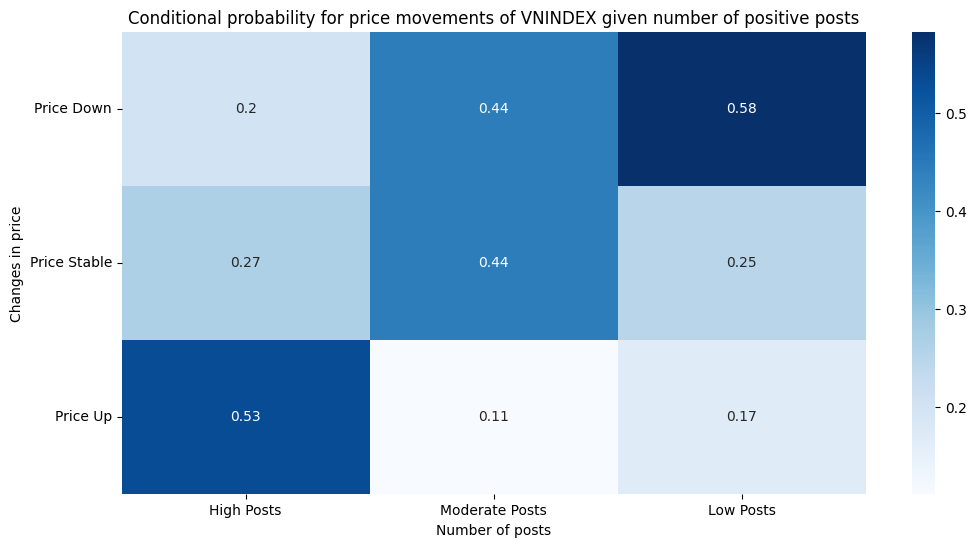
\includegraphics[width=0.9\linewidth]{images/plot-5.3-hmvnipos.png}
    \caption{Heatmap Xác suất sự thay đổi của VNINDEX dựa trên Số bài đăng Tích cực hàng ngày}
    \label{fig:5.3}
\end{figure}

Với trường hợp tích cực, xu hướng được biểu diễn tương đối rõ ràng. Xác suất chỉ ra rằng VNINDEX sẽ có khả năng tăng giá cao khi có nhiều bài Tích cực, và càng trở nên khó đoán định khi số lượng bài Tích cực giảm dần. Khi số lượng bài Tích cực càng ít, thì xu hướng giảm giá sẽ lộ càng rõ. Tựu chung, xác suất giảm giá sẽ tăng khi số lượng bài viết Tích cực giảm.\\

Nhìn chung, từ cả 3 biểu đồ, ta có thể đưa ra nhận xét rằng, các xu hướng trên đều đúng với giả thuyết, rằng tâm lý của các nhà đầu tư, thể hiện qua số lượng bài đăng trong ngày, có sự tương quan tương đối với diễn biến của thị trường thực tế trong ngày đó. Khi sử dụng số lượng bài viết Tích cực/Tiêu cực để đánh giá, xu hướng sẽ hiện ra rõ rệt hơn so với việc sử dụng số lượng bài viết chung. Đồng thời, ta nhận thấy xu hướng giảm giá sẽ biểu lộ rõ rệt hơn so với xu hướng tăng giá, một phần lý do có thể đến từ việc dữ liệu đầu vào biến động nghiêng về phía giảm nhiều hơn.

\subsubsection*{Nhận xét Phương pháp trên Toàn bộ mã cổ phiếu}

Để thực hiện được điều này, trước hết ta cho chạy hàm \texttt{bayesProbPosts} cho từng mã chứng khoán. Sau đó, với từng trường hợp kết quả, ta tính trung bình giá trị của trường hợp kết quả đó trong toàn bộ mã chứng khoán.

 \begin{figure}[H]
    \centering
    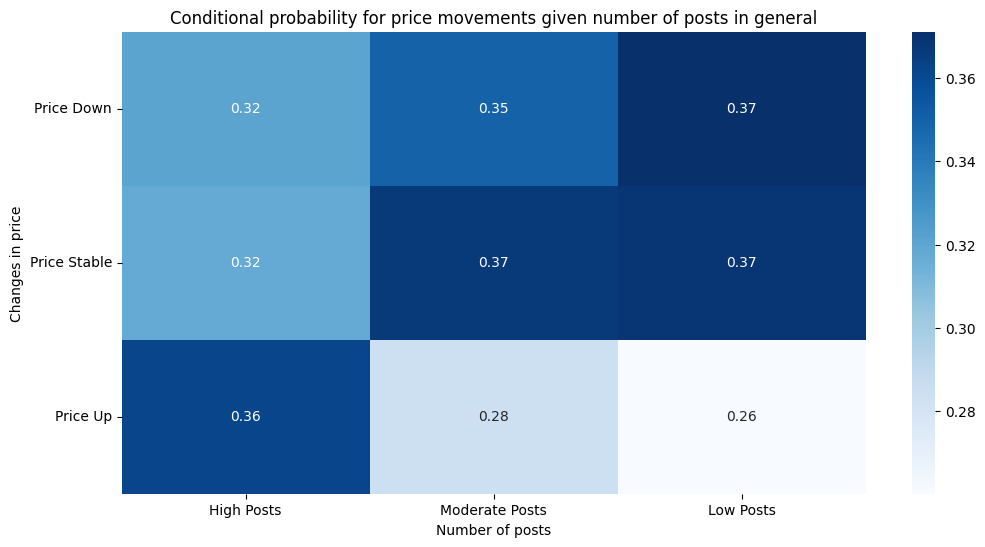
\includegraphics[width=0.9\linewidth]{images/plot-5.4-hmgenall.png}
    \caption{Heatmap Xác suất của Toàn bộ cổ phiếu dựa trên Số bài đăng hàng ngày}
    \label{fig:5.4}
\end{figure}

Điểm đặc biệt của biểu đồ (\ref{fig:5.4}) là xác suất rất đều, khi toàn bộ các trường hợp chỉ khác nhau chưa tới 9\%. Điều này khẳng định luận điểm rằng khi sử dụng số lượng bài viết chung để tính xác suất, xu hướng thị trường sẽ không lộ rõ.\\

Xu hướng đã lộ rõ hơn ở biểu đồ (\ref{fig:5.5}), và xác suất giảm giá vẫn đi xuống khi số lượng bài viết Tiêu cực giảm. Tuy nhiên, điều này không thể hiện rõ bằng biểu đồ (\ref{fig:5.2}), khi ta xét trên VNINDEX.\\

Cuối cùng là biểu đồ (\ref{fig:5.6}). Nhìn chung những luận điểm từ trước của ta vẫn chính xác.\\

Từ 3 biểu đồ heatmap trên, có thể thấy việc gộp chung dữ liệu từ tất cả các mã không phải là một phương án tối ưu, khi mà xác suất để giá trị cổ phiếu tăng, giảm hoặc duy trì ổn định đều không quá chắc chắn, dù nó vẫn thỏa mãn những luận điểm khi ta xét trên VNINDEX. Sẽ tốt hơn nếu ta thực hiện chọn lọc các cổ phiếu có xác suất tăng giảm rõ ràng hơn để tính toán. \\

\textbf{Nhận xét chung về phương pháp dự đoán giá cổ phiếu sử dụng định luật Bayes:} Mặc dù cho nhiều kết quả khả quan, tuy nhiên phương pháp này gần như không mang lại giá trị thực tiễn, do xác suất tăng hay giảm cụ thể là chưa đáng kể. Ngoài ra, ta cũng đang dùng số lượng bài đăng để dự đoán sự tăng/giảm của cổ phiếu trong ngày, nhưng giá trị cổ phiếu có biến động (tăng/giảm) thì số lượng bài đăng mới tăng. \textbf{Số lượng bài đăng trên diễn đàn không phải nguyên nhân chính khiến giá biến động}. Dẫu vậy, ta có thể dùng số lượng bài đăng như một hình thức tham khảo hoặc loại cảnh báo. 

\begin{figure}[H]
    \centering
    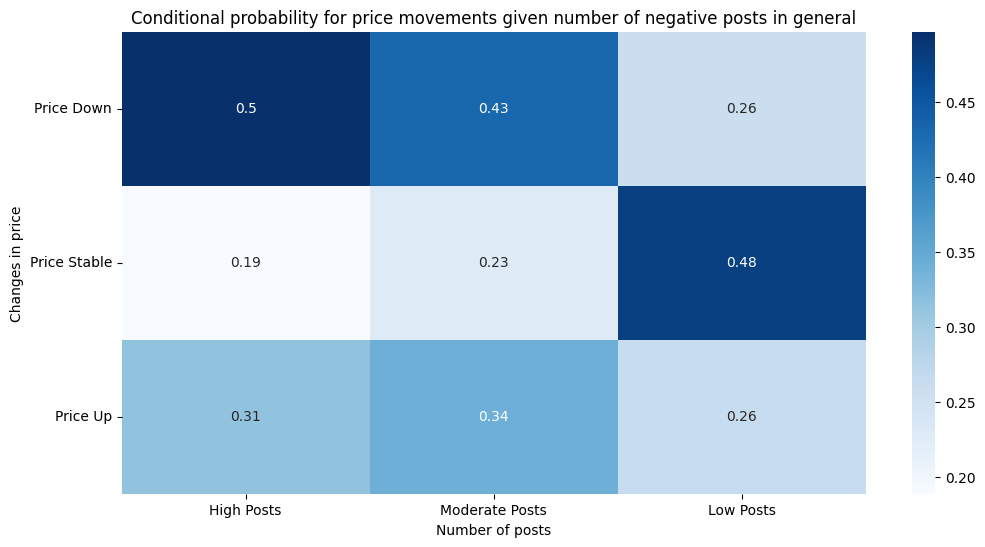
\includegraphics[width=0.9\linewidth]{images/plot-5.6-hmgenneg.png}
    \caption{Heatmap Xác suất của Toàn bộ cổ phiếu dựa trên Số bài đăng Tiêu cực hàng ngày}
    \label{fig:5.5}
\end{figure}

\begin{figure}[H]
    \centering
    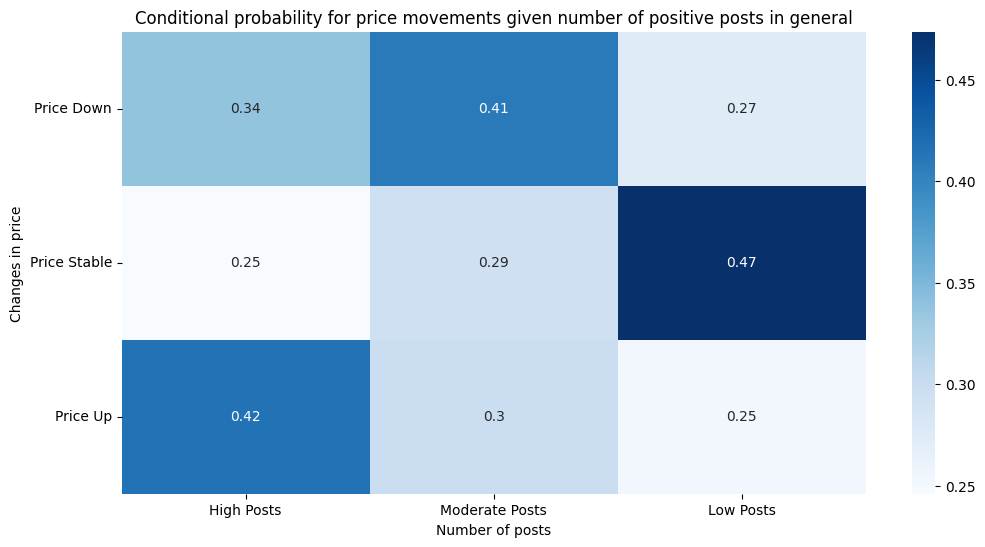
\includegraphics[width=0.9\linewidth]{images/plot-5.5-hmgenpos.png}
    \caption{Heatmap Xác suất của Toàn bộ cổ phiếu dựa trên Số bài đăng Tích cực hàng ngày}
    \label{fig:5.6}
\end{figure}

\textbf{Hướng cải thiện:} Có thể bổ sung thêm dữ liệu như nội dung các bài viết, thời gian và một vài chỉ số tài chính để làm giàu đặc trưng đầu vào. Hơn nữa, ta có thể kết hợp với các mô hình học máy khác để có được độ chính xác tốt hơn. Đồng thời, cần thêm nhiều dữ liệu để giảm nhiễu và kiểm tra lại các giả định cũng như hiệu chỉnh thông số để tăng độ chính xác.

\section{Mô hình Dự đoán giá Phiên kế tiếp sử dụng Xích Markov}

Như đã trình bày về hạn chế về phương pháp dự đoán giá trị cổ phiếu áp dụng Định luật Bayes, ta sẽ thử nghiệm với cách tiếp cận sử dụng Xích Markov. Xích Markov là một quá trình ngẫu nhiên trong đó trạng thái của hệ thống tại thời điểm tiếp theo chỉ phụ thuộc vào trạng thái hiện tại, không phụ thuộc vào các trạng thái trước đó. Quá trình này được đặc trưng bởi tính chất ``không nhớ'' (memoryless property).\\

\subsection{Chuẩn bị dữ liệu tính toán}
Gần tương tự như phần Chuẩn bị dữ liệu tính toán sử dụng Định luật Bayes (phần 5.1.1), ta cũng sẽ có một dataframe mới, lần này với nhiều cột (features) hơn:

\texttt{time, number\_of\_posts, number\_positive\_posts, number\_negative\_posts, number\_neutral\_posts}
\texttt{open, high, low, close, volume, average\_post\_length, average\_price\_mentioned}

\begin{center}
    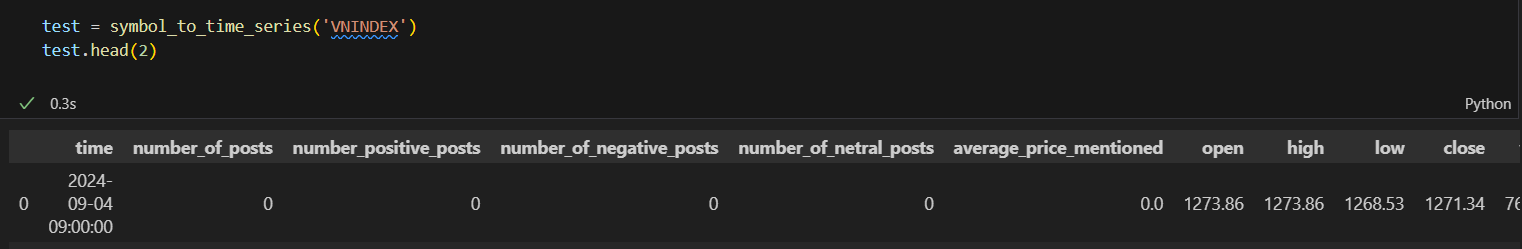
\includegraphics[width=1\linewidth]{images/C4_9.png}
\end{center}

Tương tự như phần trước, để tránh lặp lại mã nguồn cho các tính toán và thống kê tương tự nhau, ta xây dựng các hàm chức năng:

\begin{itemize}
    \item \textbf{Hàm \texttt{categorize\_posts()}}: Hàm này phân loại số lượng bài viết vào ba nhóm: cao, trung bình, hoặc thấp, dựa trên độ lệch so với số lượng bài viết trung bình.

    \item \textbf{Hàm \texttt{define\_state(change, threshold=0.01)}}: Hàm này xác định trạng thái của giá cổ phiếu là Tăng giá, Giảm giá, hoặc Ổn định giá, dựa trên ngưỡng biến động 1\%.
    
    \item \textbf{Hàm \texttt{df\_to\_transitions\_matrix(df)}}: Tạo ba ma trận chuyển trạng thái: ma trận chuyển trạng thái tổng thể, ma trận chuyển trạng thái bài viết tích cực và ma trận chuyển trạng thái bài viết tiêu cực.

    \item \textbf{Hàm \texttt{heatmap\_illustration(matrix, title, xlabel, ylabel)}}: Hàm này thực hiện trực quan hóa các ma trận chuyển trạng thái dưới dạng biểu đồ nhiệt, với các chú thích về xác suất.
\end{itemize}

\subsection{Áp dụng Xích Markov tính xác suát chuyển đổi trạng thái}

Công thức xác suất chuyển trạng thái trong xích Markov được mô tả như sau:

\[
P(X_{t+1} = j \mid X_t = i) = P_{ij}
\]

Trong đó:
\begin{itemize}
    \item \( P_{11} \) là xác suất chuyển từ Tăng giá sang Tăng giá,
    \item \( P_{12} \) là xác suất chuyển từ Tăng giá sang Giảm giá,
    \item \( P_{13} \) là xác suất chuyển từ Tăng giá sang Ổn định giá, và tương tự cho các phần tử còn lại.
\end{itemize}

Trong trường hợp phân tích cổ phiếu, ta có thể xem xét ba trạng thái chính của giá cổ phiếu: \textbf{Tăng giá}, \textbf{Giảm giá}, và \textbf{Ổn định giá}. Các trạng thái này có thể được xác định dựa trên mức thay đổi giá cổ phiếu trong một khoảng thời gian nhất định, ở đây là 1 ngày.\\

Ta có thể xây dựng ma trận chuyển trạng thái \( P \) của xích Markov, trong đó mỗi phần tử \( P_{ij} \) là xác suất chuyển từ trạng thái \( i \) sang trạng thái \( j \). Ma trận này có thể được xác định từ dữ liệu lịch sử giá cổ phiếu, ví dụ, thông qua việc tính toán tần suất xuất hiện của sự chuyển đổi giữa các trạng thái:

\[
P = \begin{pmatrix} 
P_{11} & P_{12} & P_{13} \\
P_{21} & P_{22} & P_{23} \\
P_{31} & P_{32} & P_{33} 
\end{pmatrix}
\]

Trong đó:
\begin{itemize}
    \item \( P_{11} \) là xác suất chuyển từ Tăng giá sang Tăng giá,
    \item \( P_{12} \) là xác suất chuyển từ Tăng giá sang Giảm giá,
    \item \( P_{13} \) là xác suất chuyển từ Tăng giá sang Ổn định giá, và tương tự cho các phần tử còn lại.
\end{itemize}

\subsection{Kiểm chứng Phương pháp}
Ta sẽ lập ma trận chuyển đổi của xích Markov với giá trị của VNINDEX, cho 4 trường hợp sau.

\begin{figure}[H]
    \centering
    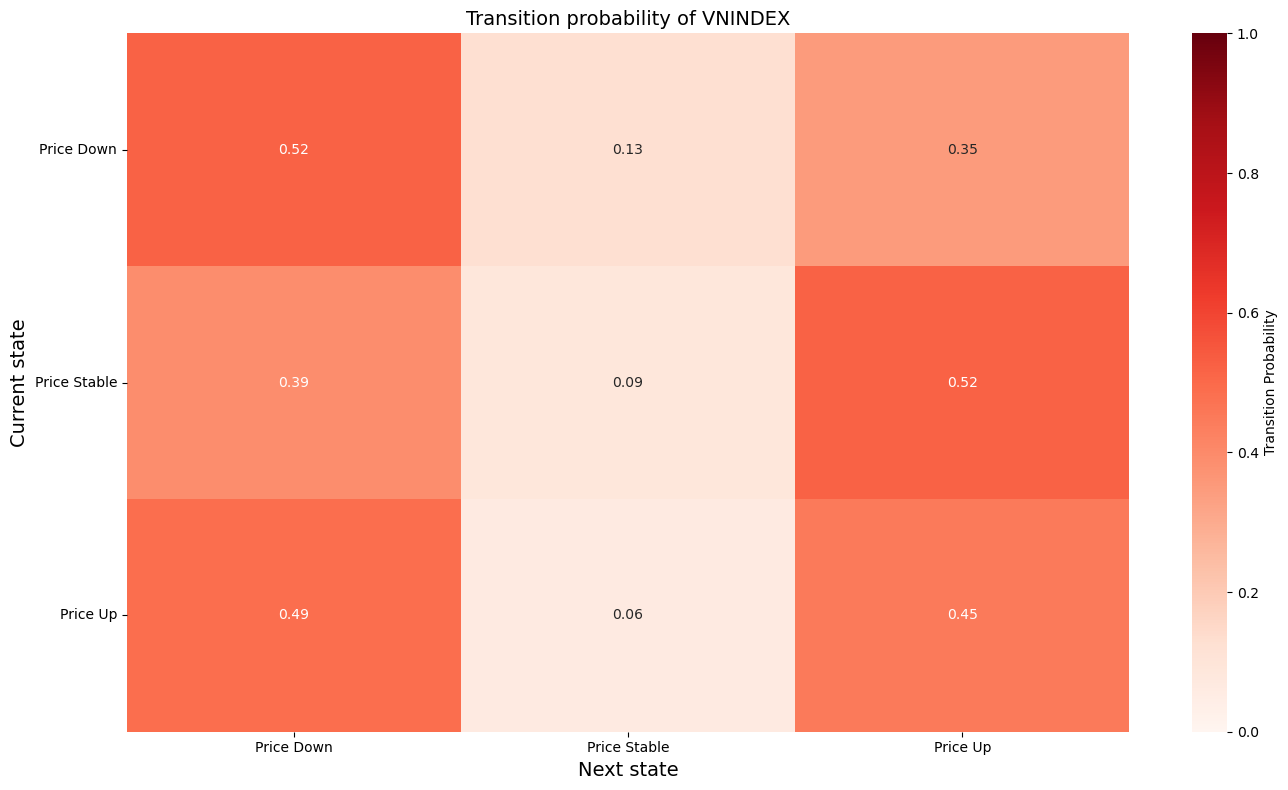
\includegraphics[width=0.9\linewidth]{images/C2_pic10.png}
    \caption{Heatmap Xác suất chuyển đổi trạng thái của giá trị VNINDEX}
    \label{fig:5.7}
\end{figure}

Dễ thấy xác suất để giá trị VNINDEX chuyển từ trạng thái hiện tại sang trạng thái tăng hoặc giảm, nhìn chung đều không chắc chắn, xoay quanh 50\%. Đơn giản là vì ta chưa xét các yếu tố nào khác mà chỉ dựa hoàn toàn lịch sử thay đổi giá trị trước đó.

\begin{figure}[H]
    \centering
    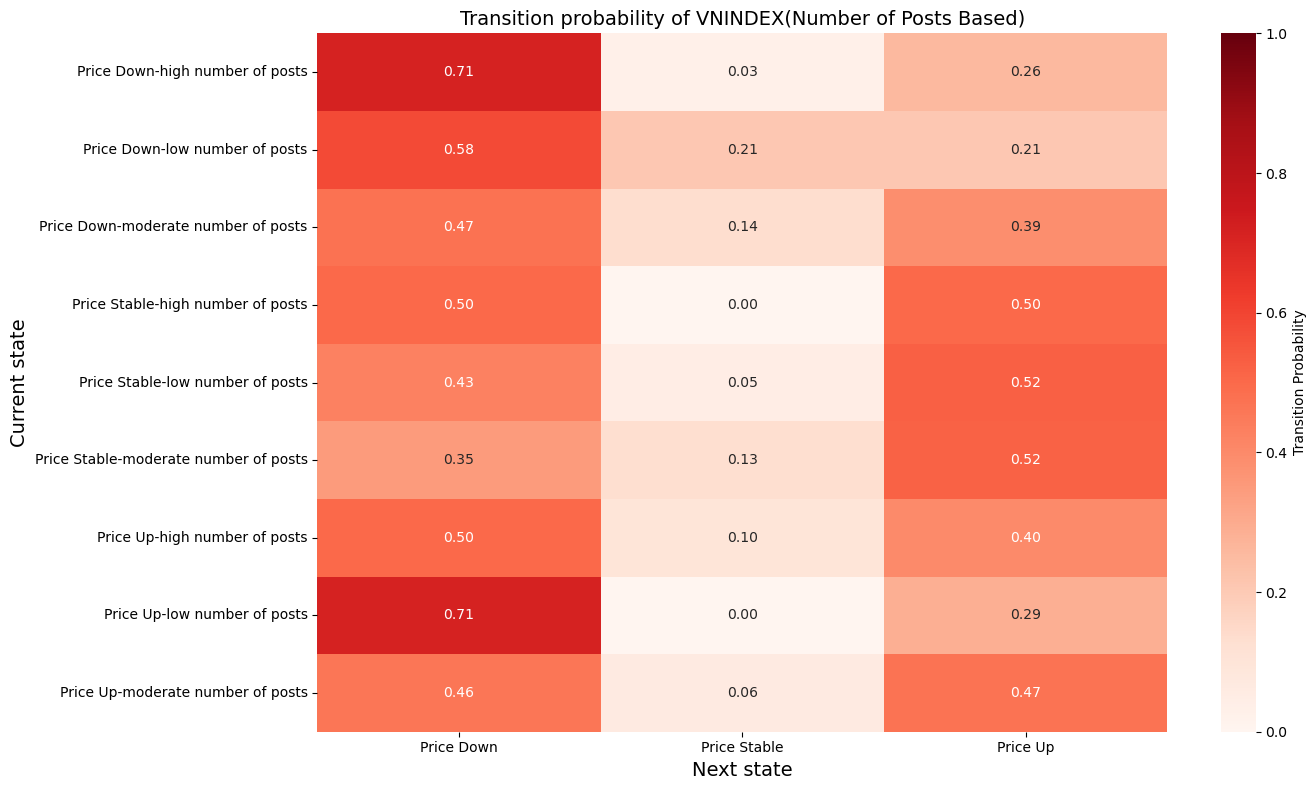
\includegraphics[width=0.95\linewidth]{images/C2_pic11.png}
    \caption{Heatmap Xác suất chuyển đổi giá trị VNINDEX (Với yếu tố Số lượng bài đăng)}
    \label{fig:5.8}
\end{figure}

Khắc phục hạn chế từ kết quả ở biểu đồ (\ref{fig:5.7}), sau khi thêm vào số lượng các bài đăng trong từng khoảng thời gian vào một trong các yếu tố thống kê, ta thu được kết quả khả quan hơn. Cụ thể, nếu ở đợt giao dịch hiện tại giá trị cổ phiếu giảm và số lượng bài viết cao, thì ở lần giao dịch tiếp theo, 71\% giá trị VNINDEX sẽ giảm. Hay giá trị cổ phiếu có khả năng giảm khoảng 71\% nếu ở đợt giao dịch hiện tại giá trị cổ phiếu tăng, số lượng bài viết thấp.

\begin{figure}[H]
    \centering
    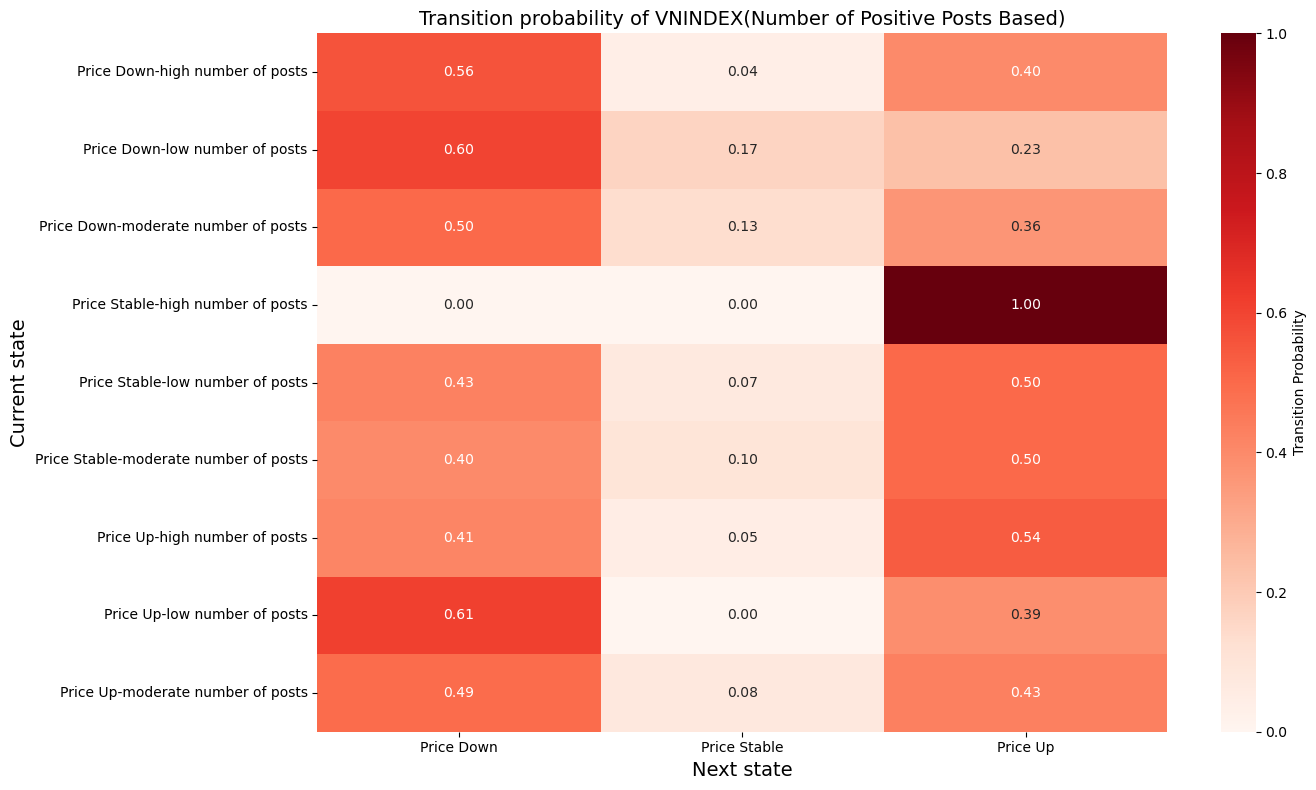
\includegraphics[width=0.95\linewidth]{images/C2_pic12.png}
    \vspace{-1em}
    \caption{Heatmap Xác suất chuyển đổi giá trị VNINDEX (Với yếu tố Số lượng bài đăng Tích cực)}
    \label{fig:5.9}
\end{figure}

Tương tự như bảng heatmap (\ref{fig:5.8}), khi số lượng bài đăng tích cực tăng cao, mà giá trị cổ phiếu lại duy trì ở mức ổn định, giá trị cổ phiếu khả năng cao sẽ tăng ở lượt giao dịch tiếp theo. Tuy vậy, trong hầu hết các trường hợp, giá trị cổ phiếu có khả năng giảm nhiều hơn tăng.

\begin{figure}[H]
    \centering
    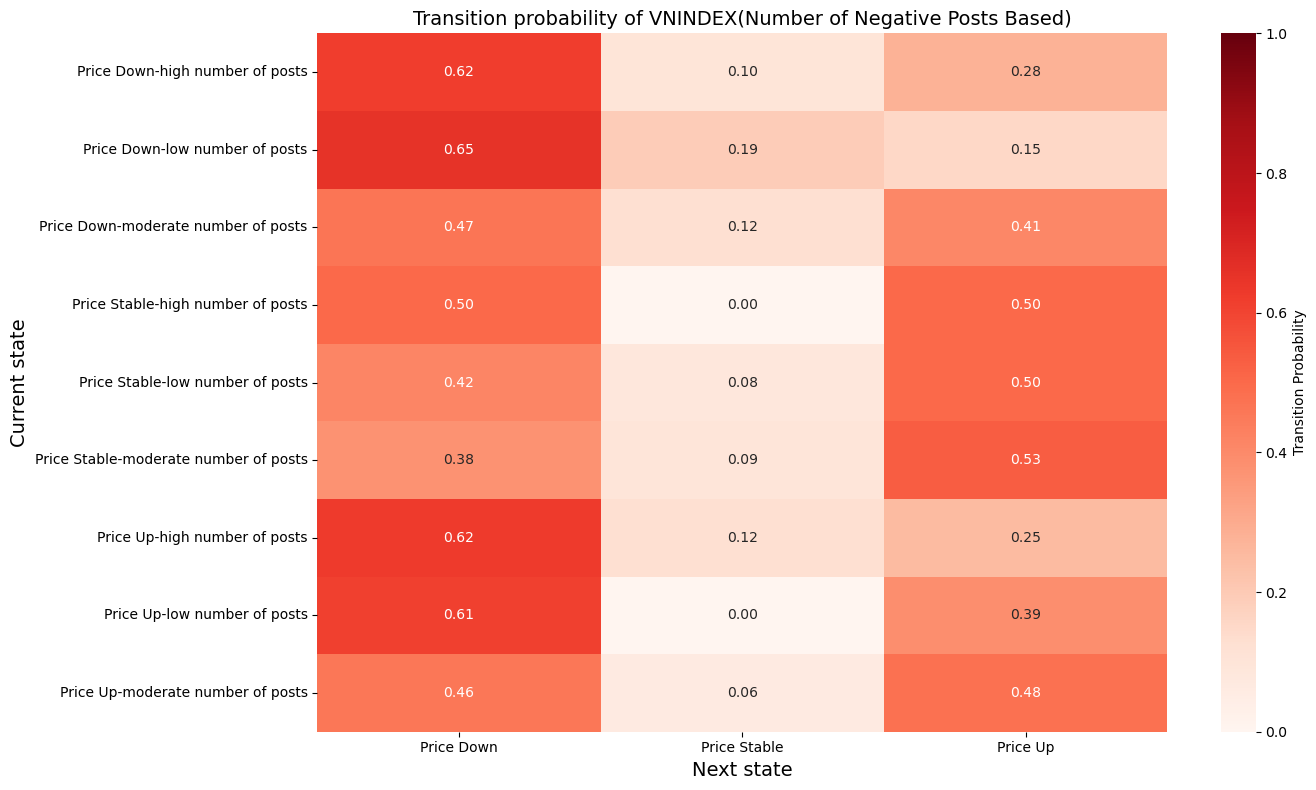
\includegraphics[width=0.95\linewidth]{images/C2_pic13.png}
    \vspace{-1em}
    \caption{Heatmap Xác suất chuyển đổi giá trị VNINDEX (Với yếu tố Số lượng bài đăng Tiêu cực)}
    \label{fig:5.10}
\end{figure}
Khác với khi sử dụng số lượng bài viết nói chung và số lượng bài viết Tích cực, khi dựa vào số bài viết Tiêu cực, ta thấy xác giá trị cố phiếu giảm chỉ cao nhất là 65\%. Điều này trái với dự đoán rằng, khi số lượng bài viết tiêu cực cao, xác suất lượt giao dịch tiếp theo giá giảm cũng sẽ cao. Tương tự xác suất chuyển đổi trạng thái sang giá trị cổ phiếu tăng cũng chỉ cao nhất là 53\% và thấp nhất là 25\%. Nhìn chung, số lượng bài viết tiêu cực không thể hiện quá nhiều về khả năng tăng hoặc giảm của mã cố phiếu sau này.\\

\textbf{Nhận xét chung về phương pháp dự đoán giá sử dụng xích Markov:} Dẫu mang lại nhiều kết quả tích, Xích Markov vẫn tồn tại nhiều hạn chế. Cụ thể, một trong những nhược điểm lớn của phương pháp xích Markov trong dự đoán giá cổ phiếu là sự giả định về tính độc lập của các trạng thái, tức là mỗi trạng thái chỉ phụ thuộc vào trạng thái ngay trước đó mà không tính đến các yếu tố dài hạn hay các biến động ngoại lai. Điều này có thể dẫn đến việc bỏ qua các yếu tố quan trọng như tin tức, sự kiện vĩ mô, hay tâm lý thị trường, vốn có thể ảnh hưởng mạnh mẽ đến biến động giá cổ phiếu. \\

Thêm vào đó, phương pháp này không thể dự đoán chính xác trong các thị trường biến động mạnh hoặc khi có những sự kiện bất ngờ, vì mô hình chỉ dựa vào dữ liệu lịch sử mà không thể dự đoán các yếu tố ngoài dữ liệu này. Tựu chung lại, \textbf{mô hình không thể được sử dụng để dự đoán giá của cổ phiếu.}\\

\textbf{Hướng cải thiện:} Ta có thể kết hợp xích Markov với các mô hình học máy phức tạp hơn, như mạng nơ-ron, hoặc cây quyết định, để tận dụng thêm các yếu tố ngoài lịch sử giá và số lượng bài đăng, chẳng hạn như dữ liệu tin tức, các chỉ số kinh tế vĩ mô, hoặc cảm xúc thị trường. Việc sử dụng các dữ liệu không phải chuỗi thời gian này có thể giúp mô hình nhận diện các yếu tố tác động dài hạn và các sự kiện ngoại lệ mà xích Markov không thể mô phỏng được. Hơn nữa, việc bổ sung các tính năng như phân tích xu hướng hoặc các chỉ số kỹ thuật có thể cải thiện độ chính xác của dự đoán, đặc biệt trong các giai đoạn thị trường thay đổi mạnh. 



\section{Mô hình Học máy Phân tích Quan điểm dựa trên Nội dung Bài viết (Sentiment Analysis) sử dụng Random Forest}
Với tập dữ liệu là những bài viết của người dùng, một khía cạnh thú vị mà ta có thể áp dụng máy học chính là phân tích quan điểm của bài viết. Ta sẽ sử dụng Học máy, cùng những kỹ thuật trong Xử lý ngôn ngữ tự nhiên nhằm tối ưu độ chính xác của kết quả.\\

Ta sẽ sử dụng thư viện Scikit-learn (\texttt{sklearn}) nhằm thực hiện những tác vụ liên quan đến Học máy. Thư viện \texttt{pandas} vẫn được sử dụng để làm việc với dữ liệu.

\subsection{Chuẩn bị dữ liệu}
Dữ liệu gốc của ta là dữ liệu của toàn bộ 270 nghìn bài viết, với hàng chục cột dữ liệu. Tuy nhiên ta chỉ quan tâm đến hai cột: nội dung bài viết (\texttt{originalContent}) và cột Quan điểm (\texttt{sentiment}).\\

Ta sẽ không lấy những bài có quan điểm Trung lập (\texttt{sentiment = 0}), do ta đang tìm cách để tạo mô hình phân loại một bài là Tích cực, hay Tiêu cực. Tiếp theo, ta sẽ bỏ những bài có gán link, do nó làm loãng dữ liệu và không đem lại giá trị khi phân định quan điểm. Sau quá trình xử lý nội dung trong bài, ta sẽ tiếp tục loại bỏ bài có độ dài $\le 5$.

\begin{center}
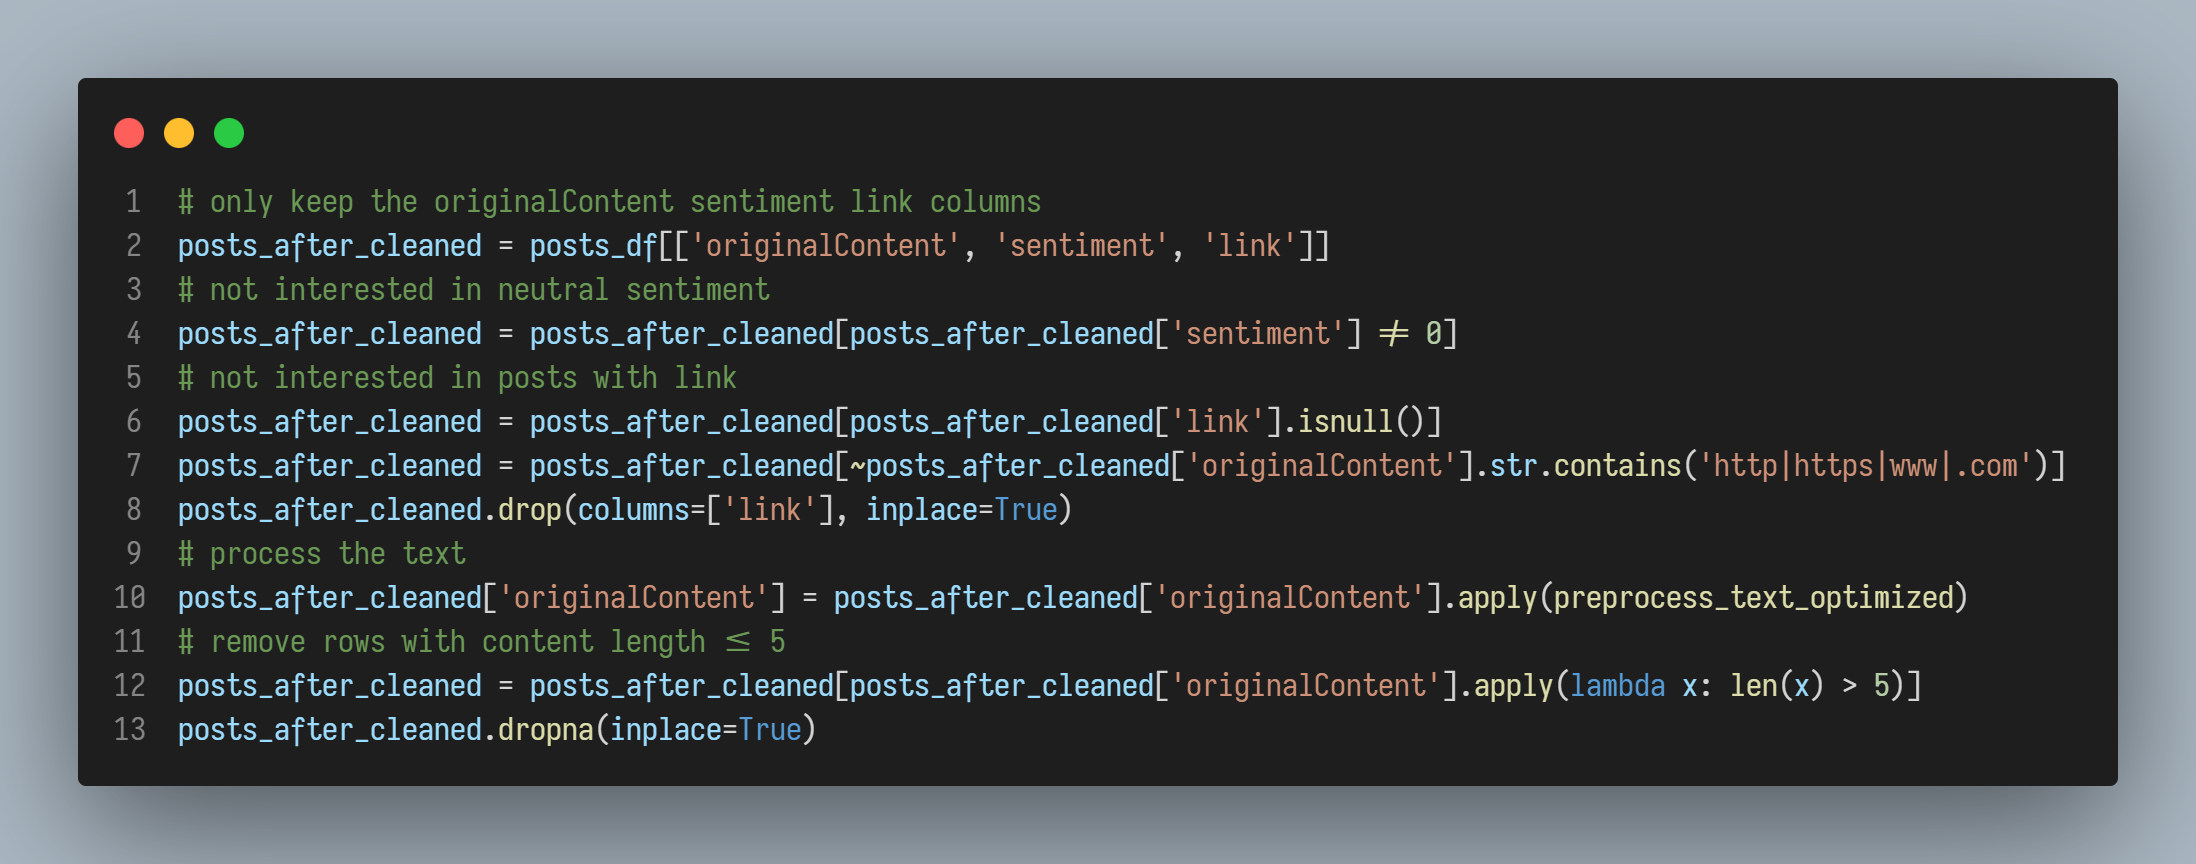
\includegraphics[width=0.8\textwidth]{images/code-5.6.png}
\end{center}

Về nội dung trong bài, trước hết ta sẽ biến mọi chữ về dạng in thường. Tiếp theo ta sẽ thực hiện bỏ những dấu câu, cũng như bỏ hết các chữ số. Với một số ký tự dạng Emoji, thay vì xóa chúng, ta giả định rằng chúng cũng sẽ góp phần thể hiện quan điểm rõ ràng hơn. Vì vậy, ta sẽ biến nó về dạng chữ (miêu tả Emoji đó bằng lời).\\

Cuối cùng là công đoạn lọc stopword. Stopword là những từ không mang đậm ý nghĩa tiêu cực hay tích cực. Việc để lọt stopword sẽ ảnh hưởng xấu đến kết quả của mô hình, vậy nên ta cần lọc chúng. Ban đầu ta sẽ sử dụng một tập dữ liệu stopword chung chung \cite{vnstopwords}, rồi sẽ dần dần thêm bớt hoặc bỏ đi các từ để phù hợp với tập dữ liệu của ta.
\begin{center}
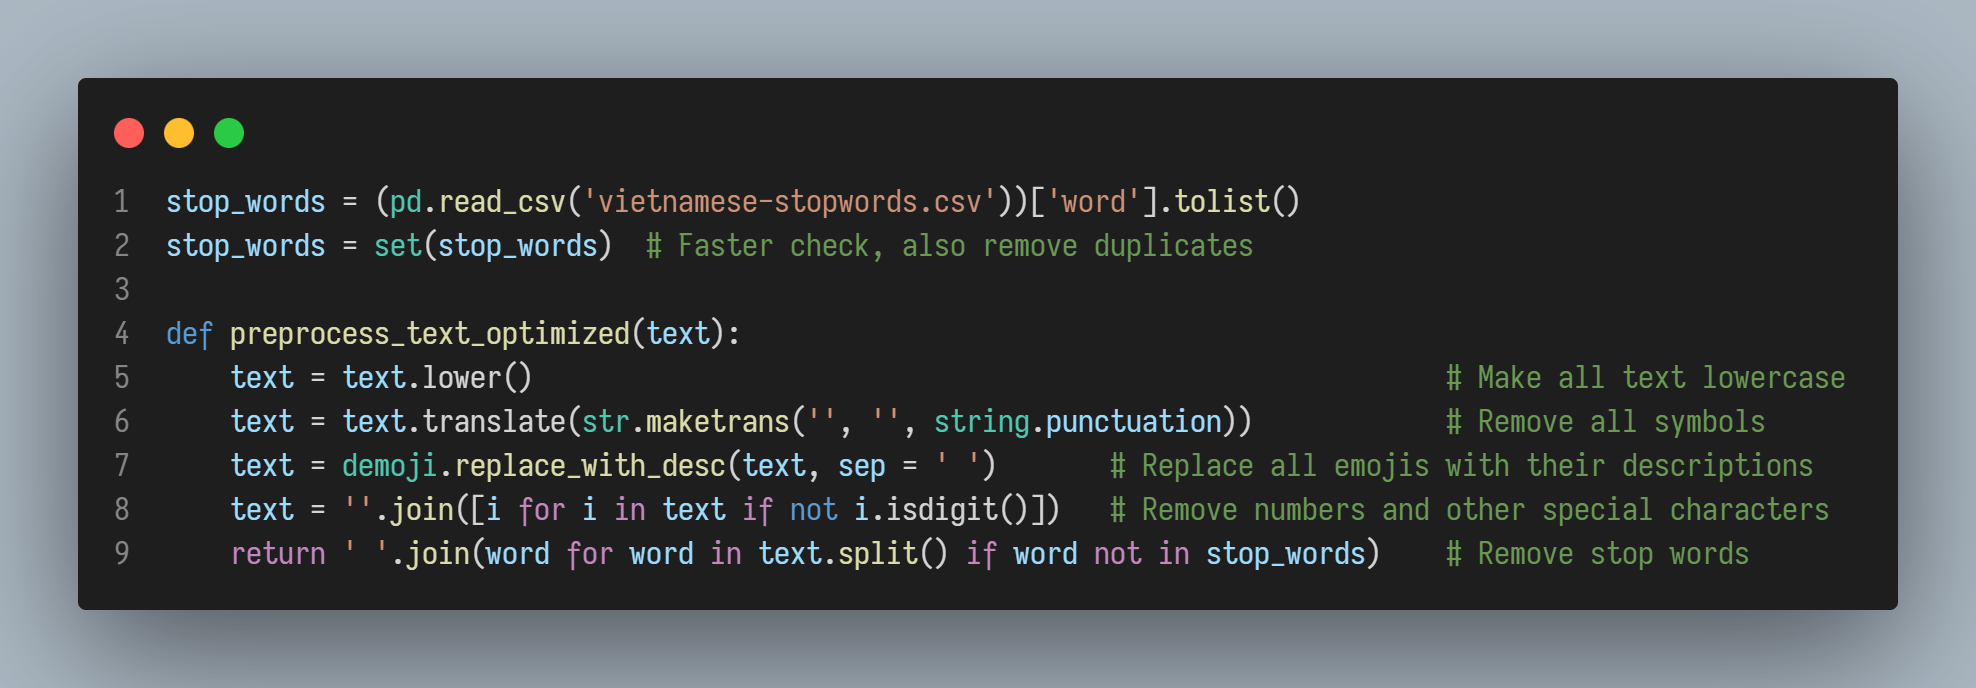
\includegraphics[width=0.78\textwidth]{images/code-5.7.png}
\end{center}

Kết quả, ta có \textbf{21159 bài Tích cực, 11771 bài Tiêu cực}. Dữ liệu này đủ đa dạng để ta tiếp tục. 
\begin{figure}[H]
  \begin{subfigure}{.5\textwidth}
  \centering
    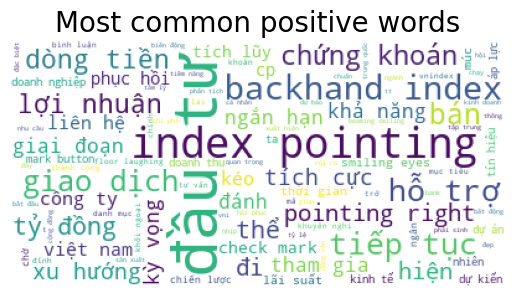
\includegraphics[width=1\linewidth]{images/plot-5.8-commonpos.png}
  \end{subfigure}%
  \begin{subfigure}{.5\textwidth}
  \centering
    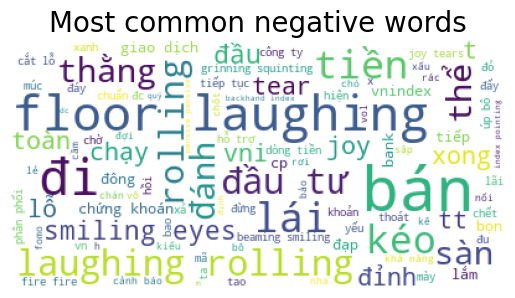
\includegraphics[width=1\linewidth]{images/plot-5.9-commonneg.png}
  \end{subfigure}
  \vspace{-2em}
  \caption{Một số từ hàm ý Tích cực và Tiêu cực xuất hiện nhiều nhất}
  \label{fig:5.11}
\end{figure}

Công đoạn tiếp theo ta sẽ thực hiện kỹ thuật TF-IDF. TF-IDF (term frequency–inverse document frequency) được dùng nhằm phản ánh tầm quan trọng của một từ đối với một văn bản trong một tập hợp hay một ngữ liệu văn bản. Ta sử dụng nó để biến văn bản thành vector chứa trọng số của các từ xuất hiện trong đoạn văn bản đó. Thư viện \texttt{scikit-learn} có chứa sẵn code cần thiết cho tác vụ này:

\begin{center}
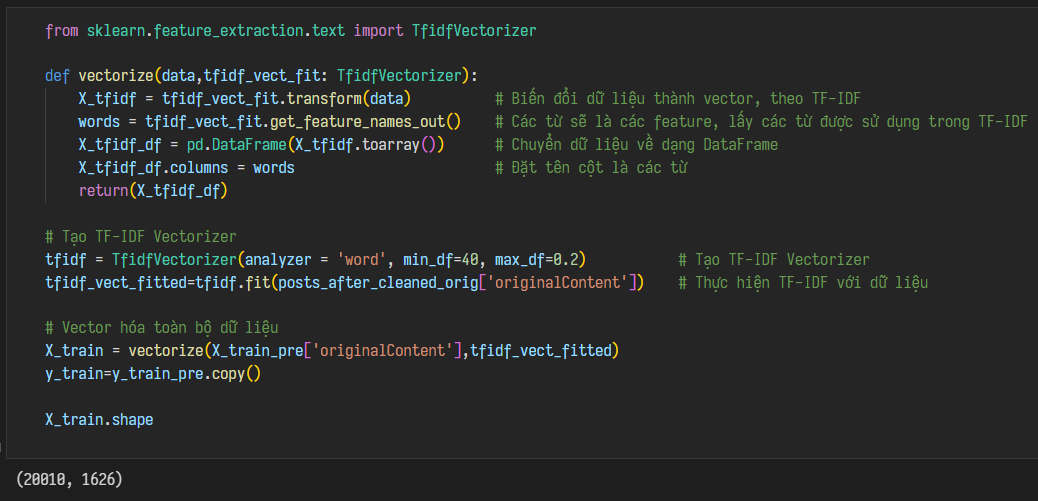
\includegraphics[width=0.8\textwidth]{images/code-5.8-tfidf.png}
\end{center}

Ta sẽ đặt các tham số cho kỹ thuật TF-IDF. Đầu tiên, ta thực hiện phân tách các từ bằng dấu cách (` '), bằng việc đặt \texttt{analyzer = `word'}. Nói cách khác ta sẽ chỉ làm việc với những từ đơn. Điều này tương đối tệ khi áp dụng với tiếng Việt, do có nhiều từ cần phải là từ ghép mới mang được đầy đủ ý nghĩa. Ta có thể tối ưu bằng việc sử dụng một Tokenizer được làm đặc biệt cho tiếng Việt, tuy nhiên với độ phức tạp của dự án, ta sẽ chỉ sử dụng phân tách bằng dấu cách.\\

Tiếp theo ta sẽ đặt ngưỡng tối thiểu để một từ được xuất hiện trong danh sách từ để xét TF-IDF là 40 lần (\texttt{min\_df = 40}); tương tự, ngưỡng tối đa là xuất hiện 20\% trong văn bản (\texttt{max\_df = 0.2}). Đặt ngưỡng tối thiểu sẽ giúp tăng độ chính xác, vì những từ xuất hiện ít ảnh hưởng không đáng kể đến kết quả, hơn nữa còn giúp huấn luyện mô hình nhanh hơn, do phải làm việc với ít từ. Đặt ngưỡng tối đa cũng sẽ ngăn tình trạng để lọt stopword, giúp thuật toán chính xác hơn. Kết quả, ta có \textbf{1626 từ được dùng} để tạo vector trọng số cho nội dung bài viết.\\

Tiếp theo ta sẽ tiến hành phân tách tập dữ liệu thành 3 phần: tập Train (85\%), tập Validation (7.5\%), và tập Test (7.5\%). Ta sử dụng hàm \texttt{train\_test\_split} trong \texttt{sklearn} để thực hiện tách tập dữ liệu:

\begin{center}
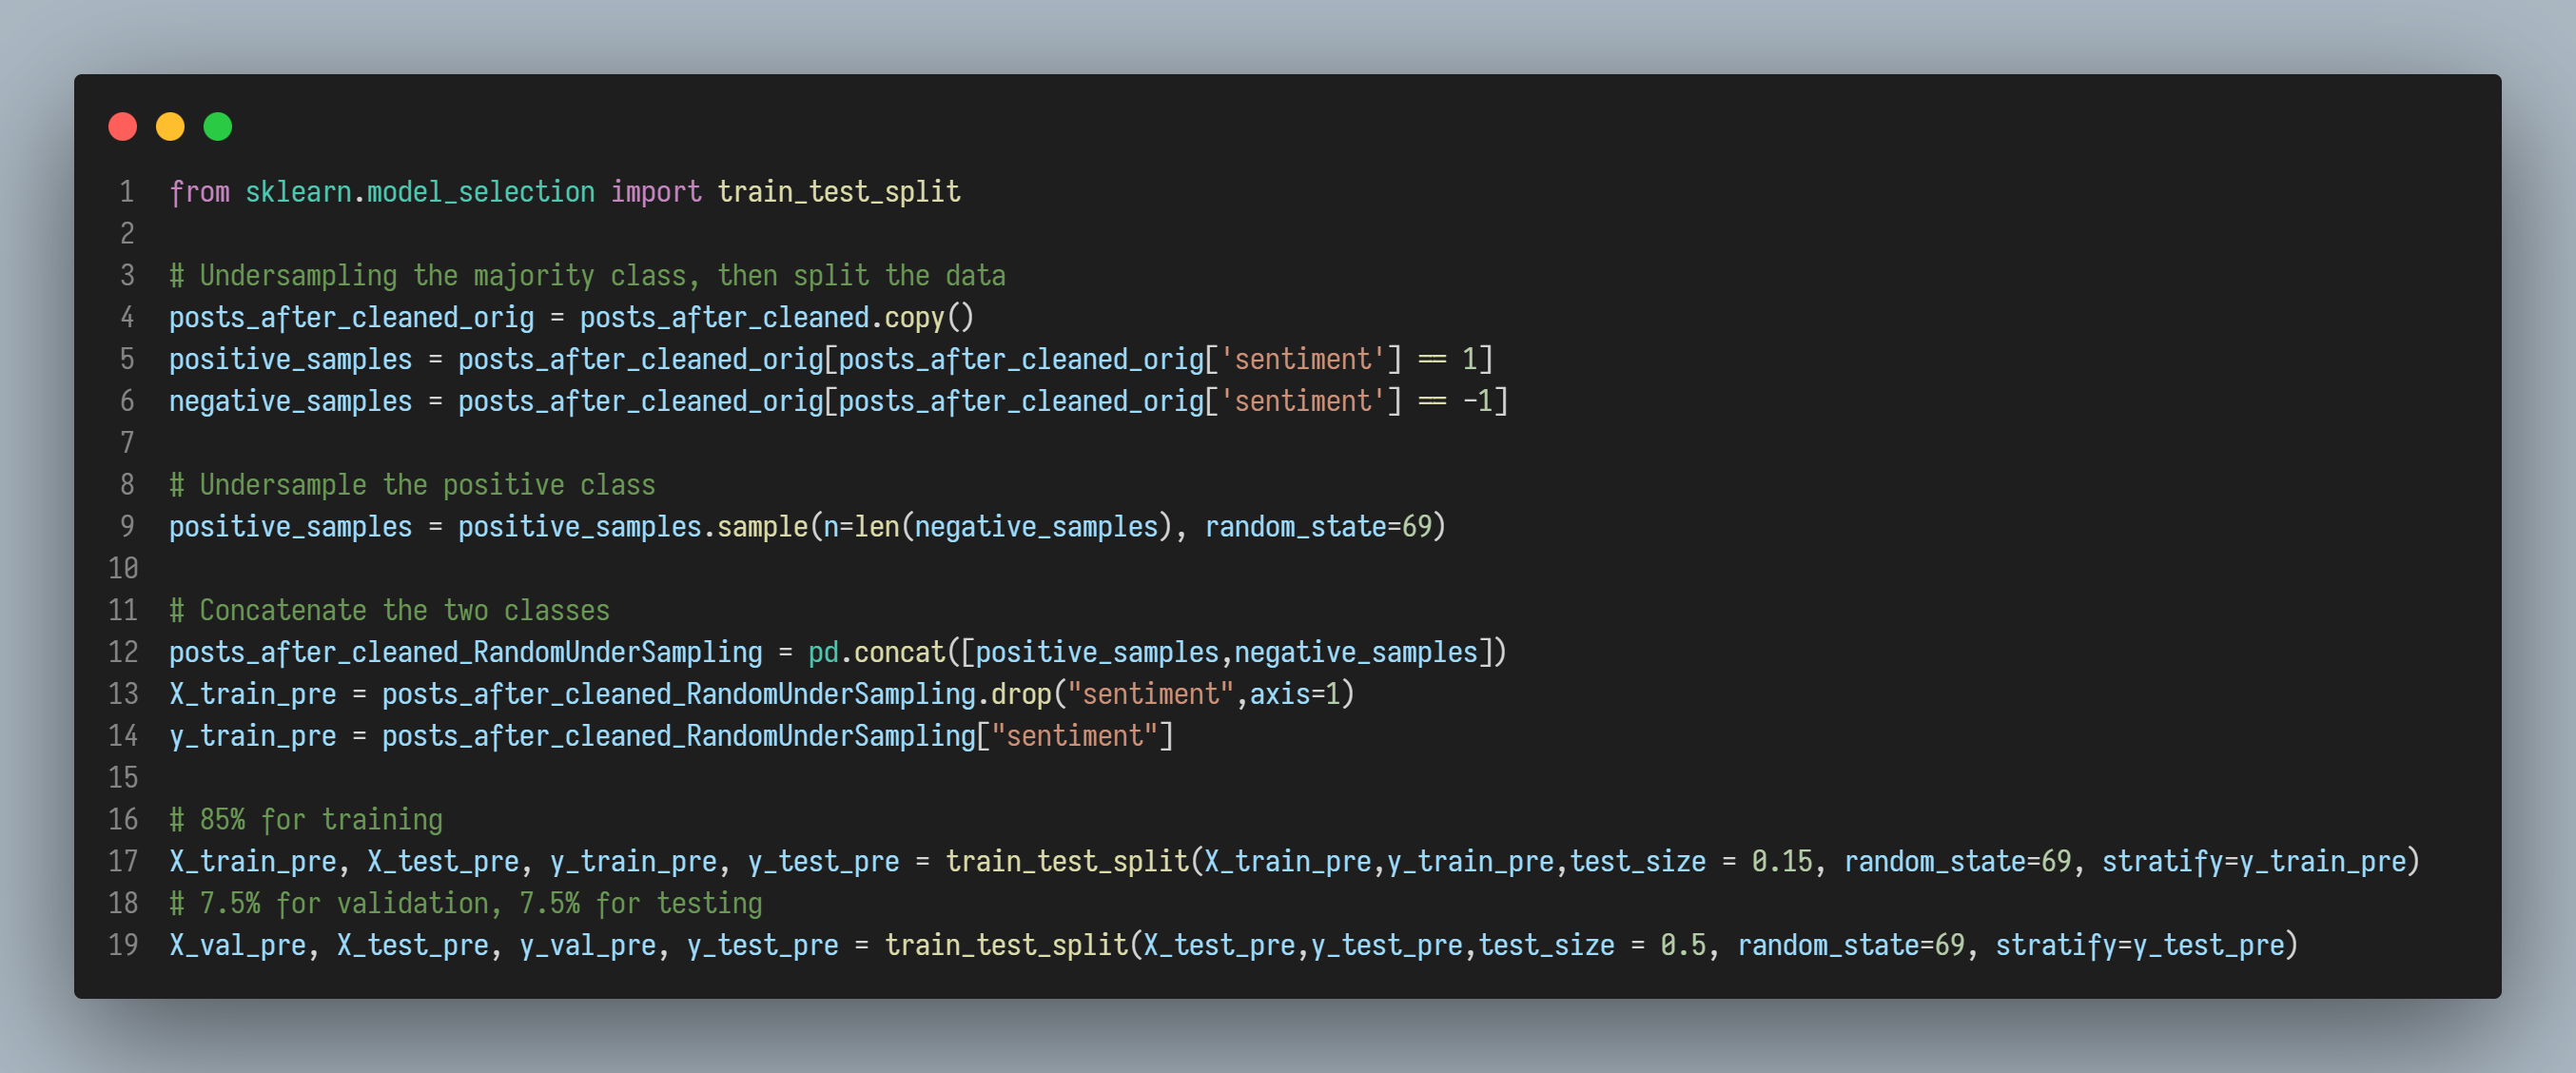
\includegraphics[width=1\textwidth]{images/code-5.9-splitdata.png}
\end{center}

Vấn đề lớn nhất của ta trong tập dữ liệu chính là sự \textbf{mất cân bằng của dữ liệu đầu vào}. Có tới 64.2\% bài viết là Tích cực trong khi chỉ có 35.8\% bài viết Tiêu cực. Sự ảnh hưởng lớn này dễ tạo ra sự thiên vị cho mô hình, đồng thời kết quả kiểm tra mô hình sẽ bị ảnh hưởng mạnh, đặc biệt với mô hình kiểu như Random Forest. Có một vài cách xử lý cho tập dữ liệu này, thậm chí còn có sẵn thư viện có thể giúp chúng ta giải quyết vấn đề (sẽ được nói ở phần 5.3.4). Ta sẽ sử dụng \textbf{phương pháp Random Under-sampling}, nghĩa là ta sẽ chọn \textbf{ngẫu nhiên} các bài Tích cực, và chọn cho tới khi số bài được chọn bằng với số bài Tiêu cực có trong tập dữ liệu.\\

Sau khi Under-sampling, số bài Tích cực bằng với số bài Tiêu cực và bằng \textbf{11771 bài}. Cuối cùng, tập Train có \textbf{20010 bài}; tập Validation và Test đều có \textbf{1766 bài}. Tất cả dữ liệu đều có tỉ lệ bài Tích cực và Tiêu cực \textbf{bằng nhau}.

\subsection{Huấn luyện mô hình}
Sau khi có dữ liệu, ta sẽ thực hiện huấn luyện cho mô hình. Ta sẽ sử dụng \textbf{mô hình Random Forest} để thực hiện tác vụ này. Sở dĩ ta sử dụng Random Forest, thứ nhất vì tính đơn giản của nó, cũng như khả năng làm việc với ma trận nhiều chiều và tập dữ liệu lớn, phù hợp với những tác vụ liên quan đến ngôn ngữ. Random Forest cũng có thể xử lý các giá trị khuyết thiếu, outliers, điều dễ có thể xảy ra trong tập dữ liệu của ta. Để kiểm chứng độ hiệu quả của mô hình, ta sẽ sử dụng kỹ thuật Cross-validation, với tiêu chí chấm điểm là độ chính xác (accuracy):

\begin{center}
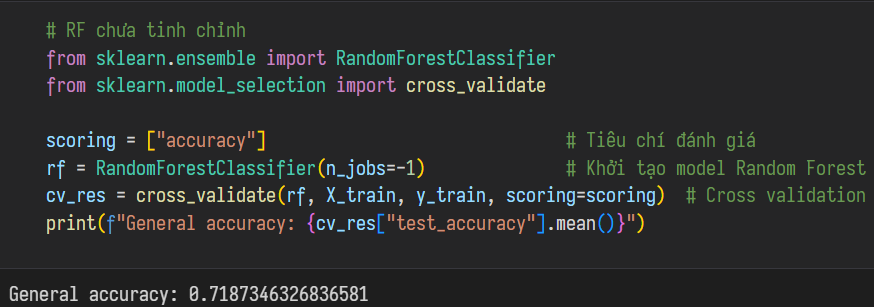
\includegraphics[width=0.7\textwidth]{images/code-5.10-rf1cv.png}
\end{center}

Kết quả khá ổn khi mô hình có độ chính xác bình quân là 71.8\% trên tập Train.\\

Tiếp theo ta sẽ tìm ra tham số tốt nhất để mô hình chạy tốt hơn. Ta sẽ sử dụng hàm \texttt{GridSearchCV} có trong \texttt{sklearn}. \texttt{GridSearchCV} sẽ thực hiện thử từng cặp tham số, sau đó đánh giá sử dụng Cross-validation để chọn ra cặp tham số hiệu quả nhất. Ta sẽ thực hiện thử với 3 loại tham số chính, là \texttt{n\_estimators} (số lượng Cây quyết định), \texttt{max\_features} (số lượng feature (đầu vào) sẽ lấy để chia cây), và \texttt{max\_depth} (độ sâu tối đa của Cây).

\begin{center}
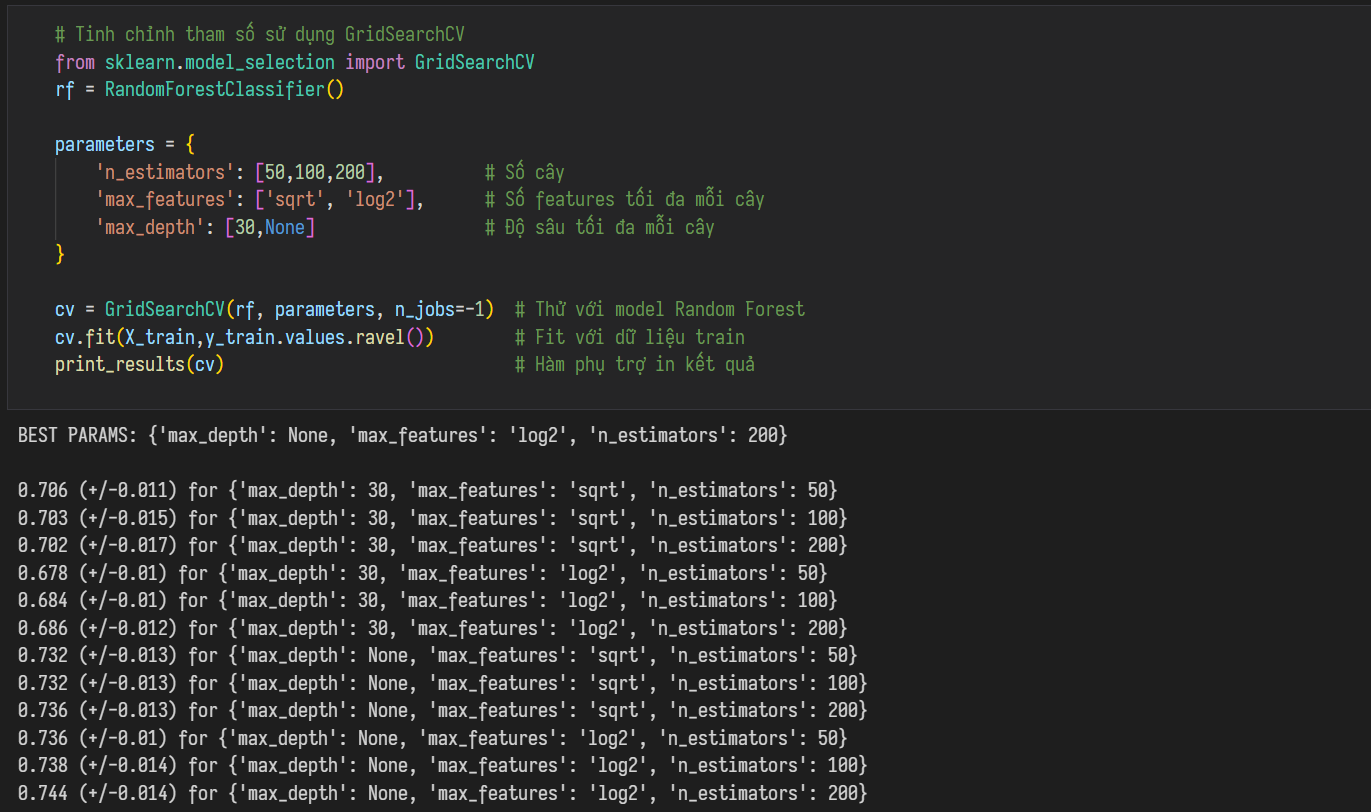
\includegraphics[width=1\textwidth]{images/code-5.11-gridsearch.png}
\end{center}

Như vậy, kết quả chỉ ra rằng, việc không giới hạn độ sâu mỗi cây, sử dụng tối đa log2 lượng feature, và có 200 cây quyết định sẽ đưa ra kết quả tốt nhất với độ chính xác 74.4\% trên tập Train.\\

Để kiểm chứng những tham số tốt nhất, ta cần thử trên tập Validation. Ta chọn ra 3 cặp tham số tốt nhất, huấn luyện chúng qua tập Train, và cho chúng thử trên tập Validation. Ngoài ra ta cũng lưu lại thời gian huấn luyện để trợ cho quyết định so sánh.

\begin{center}
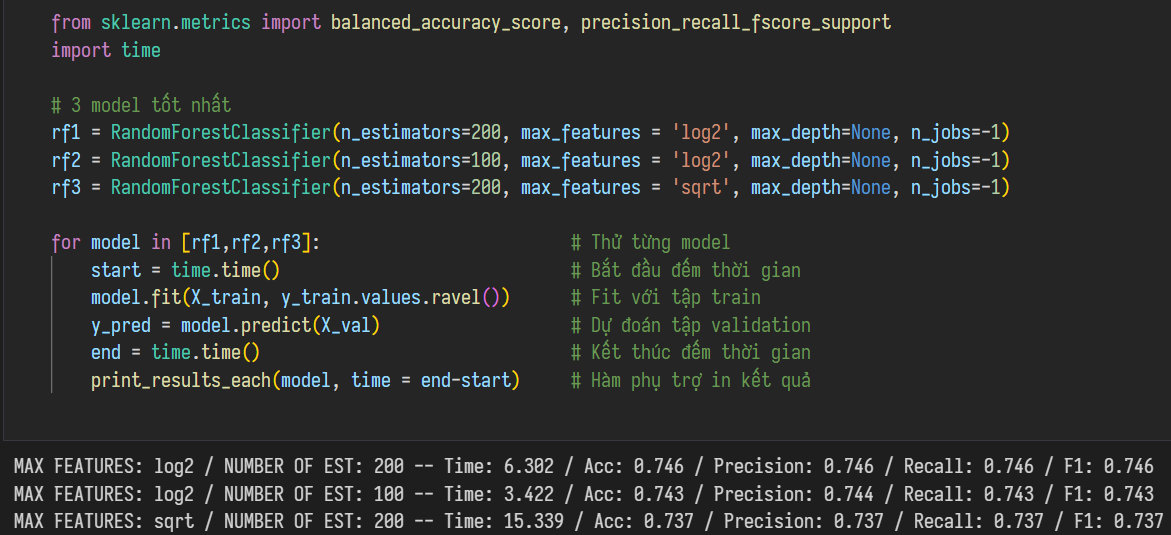
\includegraphics[width=0.9\textwidth]{images/code-5.12-rfval.png}
\end{center}

Kết quả tương đồng với dữ liệu trong tập Train, hơn nữa thời gian huấn luyện mô hình \texttt{log2} nhanh hơn hẳn so với mô hình \texttt{sqrt}. Vậy, ta sẽ sử dụng mô hình \texttt{rf1} làm mô hình chính để thử với tập Test.\\

Kết quả cuối cùng của mô hình có độ chính xác \textbf{74.2\%}, với các chỉ số recall và f1-score đều đẹp.

\begin{center}
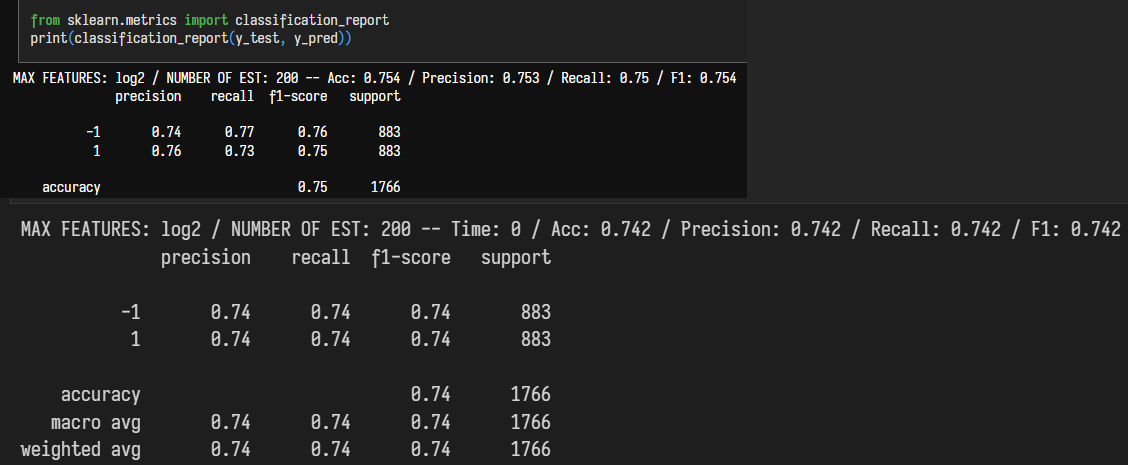
\includegraphics[width=0.9\textwidth]{images/code-5.13-rftest.png}
\end{center}

\subsection{Cải thiện dữ liệu đầu vào}
Ta có thể cải thiện dữ liệu đầu vào bằng nhiều cách. Ví dụ, ta có thể xét thêm tham số là số lượng từ chửi thề có trong đoạn văn bản. Bài nào nhiều từ chửi thề, khả năng cao sẽ mang ý Tiêu cực.

\begin{center}
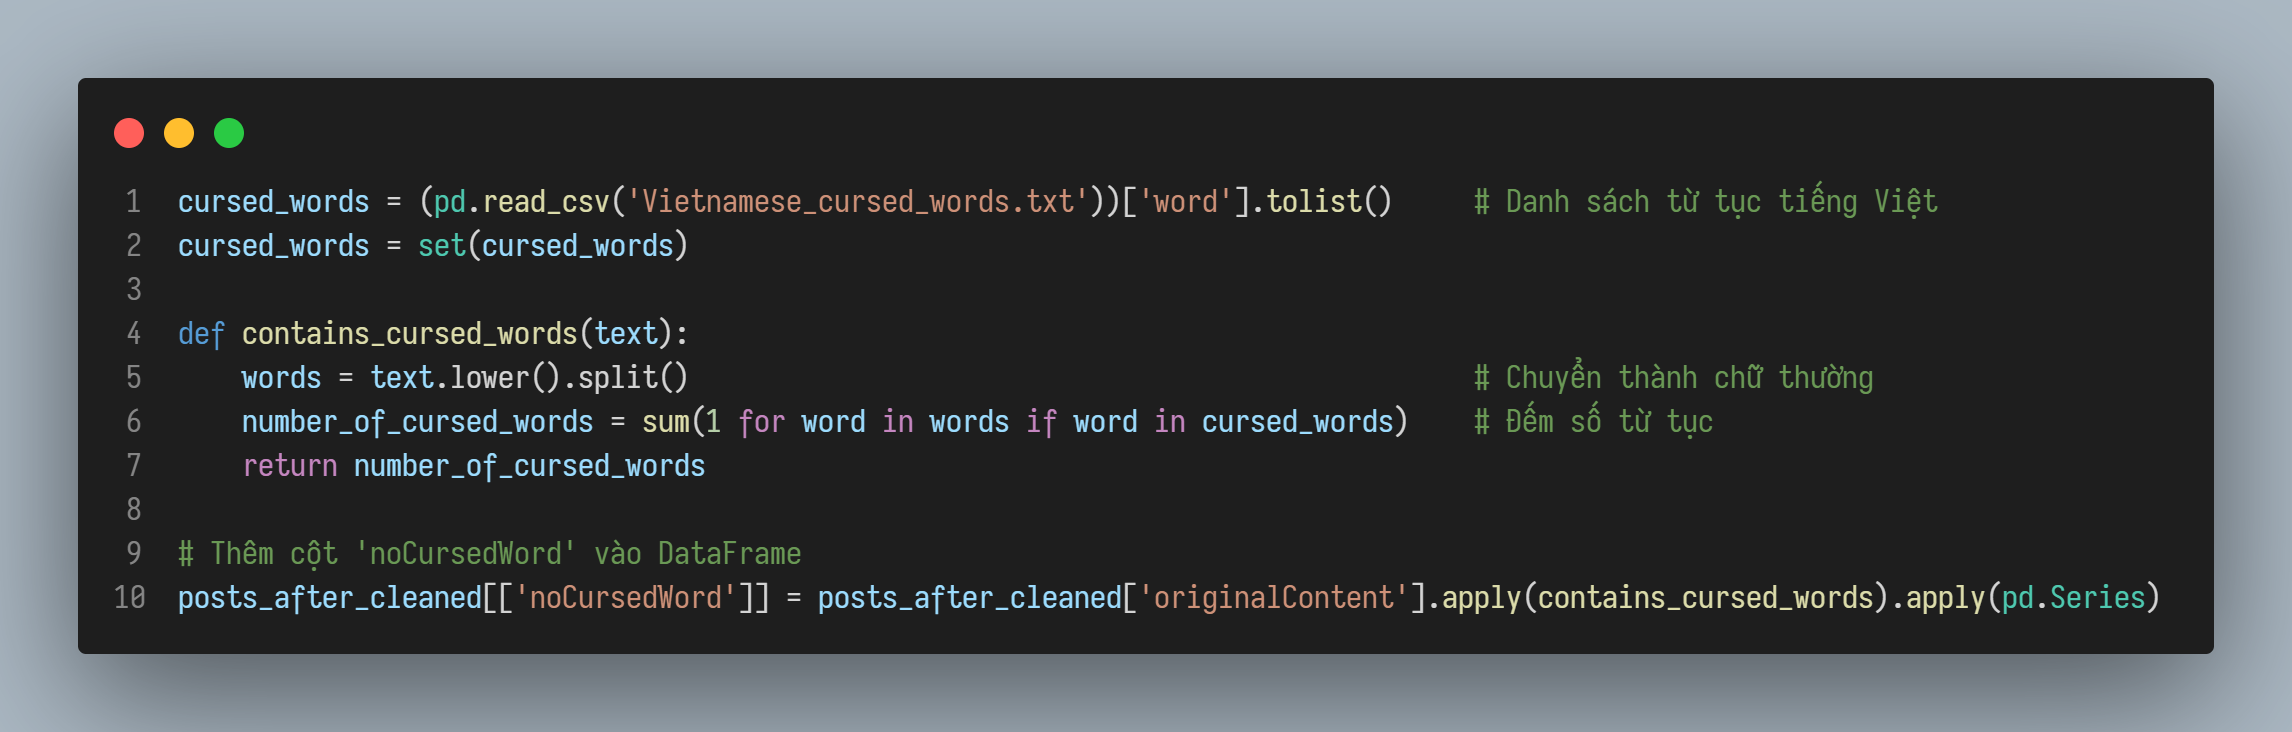
\includegraphics[width=1\textwidth]{images/code-5.14-cw.png}
\end{center}

Hơn nữa, ta có thể tinh chỉnh danh sách stopword cho phù hợp với tập dữ liệu của ta. Ta xét top 40 từ ảnh hưởng nhiều nhất đến quyết định của mô hình (hình (\ref{fig:5.12})).\\

Ta nhận thấy ngoài những từ mang hàm ý Tích cực (múc, mua, tím, trần, gom, chạy...), và những từ mang ý Tiêu cực (đi, sàn, lỗ, chốt, đạp, ...), vẫn còn xuất hiện những từ không mang nhiều ý nghĩa phân định (face, ae, hàng, phiên, hôm, nay, mai, ...). Ta sẽ thực hiện loại bỏ những từ này bằng cách thêm nó vào danh sách stopword (hình (\ref{fig:5.13})).\\

Sau khi thực hiện các cách trên, độ chính xác đã được cải thiện khá tốt, từ \textbf{74.2\%} lên \textbf{75.4\%}.

\begin{center}
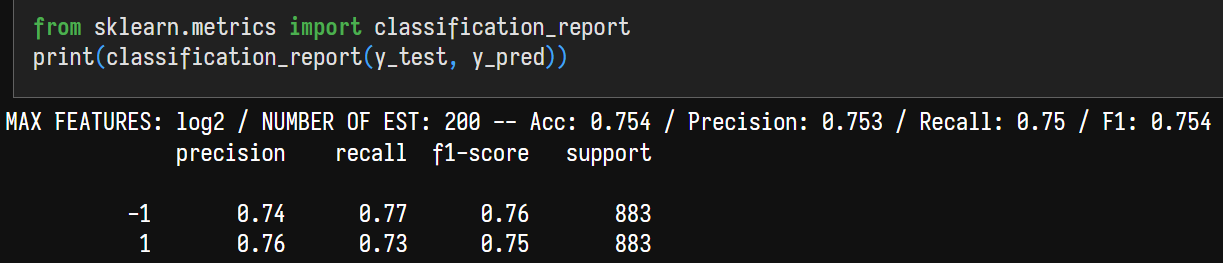
\includegraphics[width=1\textwidth]{images/code-5.15-rftestaft.png}
\end{center}

\begin{figure}[H]
    \centering
    \vspace{-2em}
    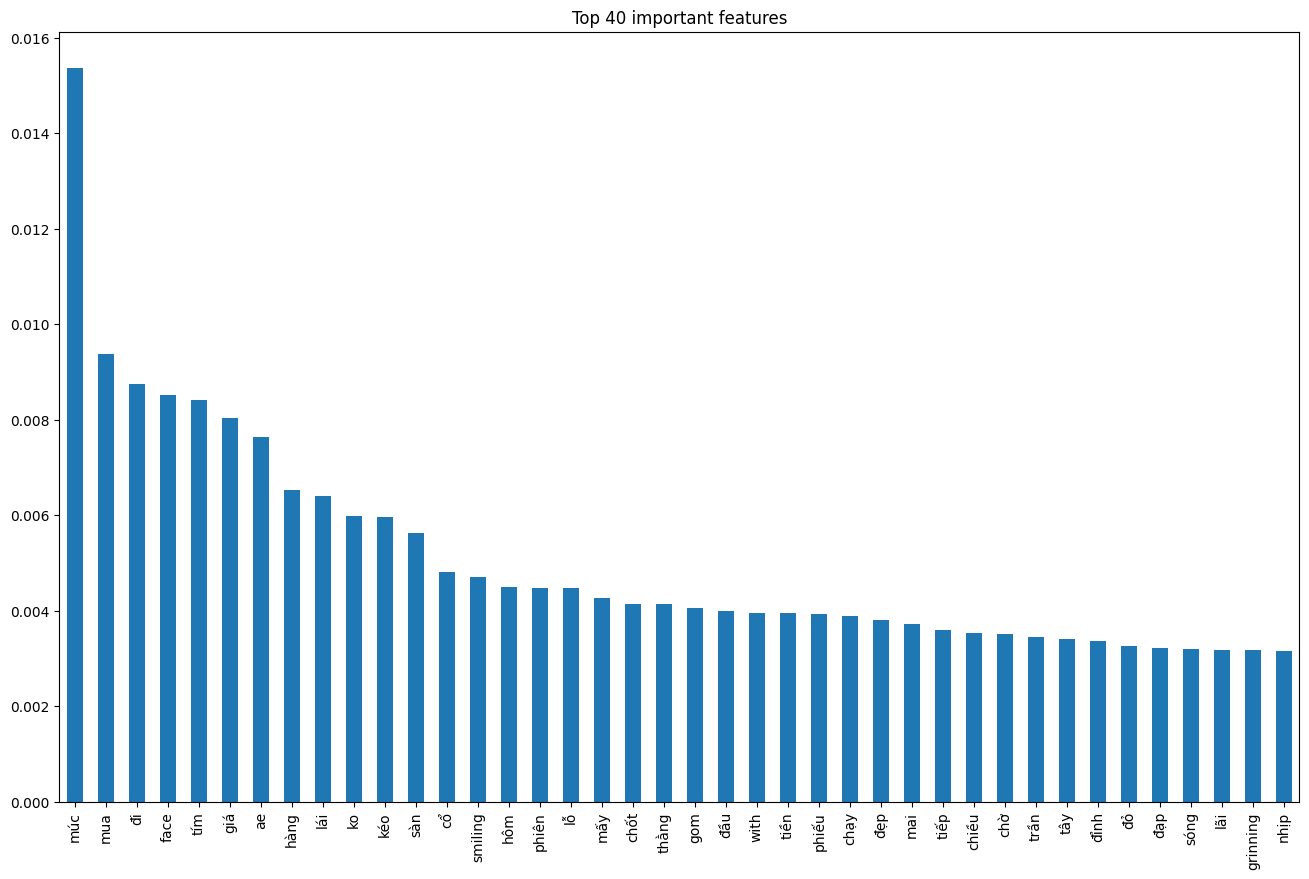
\includegraphics[width=1\linewidth]{images/plot-5.7-prefiltersw.png}
    \vspace{-2em}
    \caption{Top 40 từ ảnh hưởng nhiều nhất tới mô hình (trước khi lọc)}
    \label{fig:5.12}
\end{figure}
\vspace{-1.5em}
\begin{figure}[H]
    \centering
    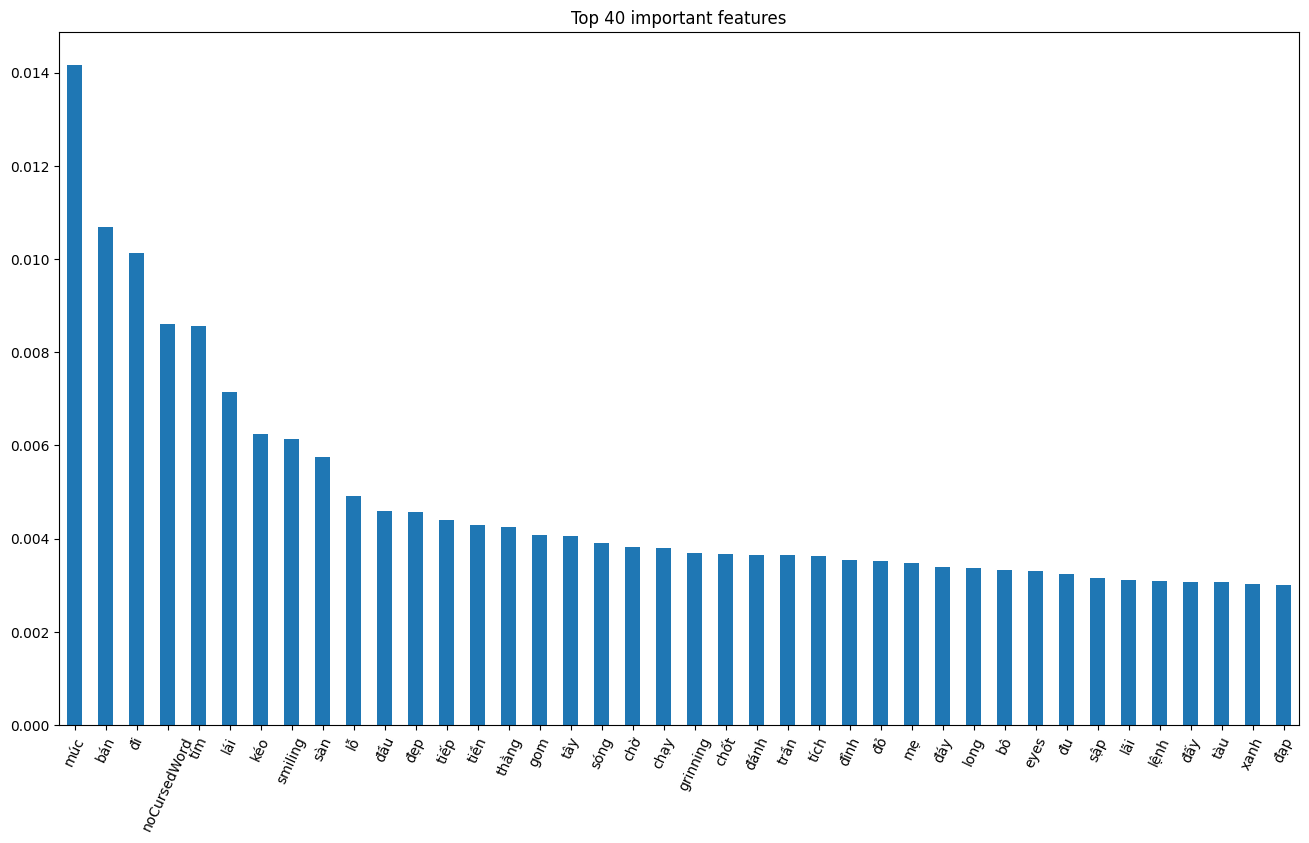
\includegraphics[width=1\linewidth]{images/plot-5.10-40featureslist.png}
    \vspace{-2.5em}
    \caption{Top 40 từ ảnh hưởng nhiều nhất tới mô hình (sau khi lọc một số từ)}
    \label{fig:5.13}
\end{figure}
\vspace{-2em}
\subsection{Sử dụng thư viện \texttt{imbalanced-learn}}
Đặc trưng dữ liệu của ta là sự thiếu cân bằng giữa số bài viết Tích cực và Tiêu cực. Để làm việc thuận tiện hơn với loại dữ liệu này, thư viện \texttt{imbalanced-learn} \cite{imblearn} ra đời, dựa trên cơ sở là thư viện \texttt{scikit-learn}. Ta sẽ thử nghiệm mô hình \texttt{BalancedRandomForestClassifier} có trong thư viện này. Bản chất của nó vẫn là Random Forest, tuy nhiên nó sẽ tự động thực hiện các bước Random Under-sampling mà không cần ta phải cài đặt.\\

Ta sẽ phân lại dữ liệu đầu vào bằng cách lấy sẵn khoảng 5\% số dữ liệu làm tập Test, và 95\% còn lại là tập Train. Như vậy tập Test có 1800 bài, còn tập Train có 31130 bài. Tập Test sẽ có số lượng bài Tích cực và Tiêu cực bằng nhau (900 bài), còn tập Train thì không. Kết quả rất ấn tượng, với \textbf{76.2\%}:
\begin{center}
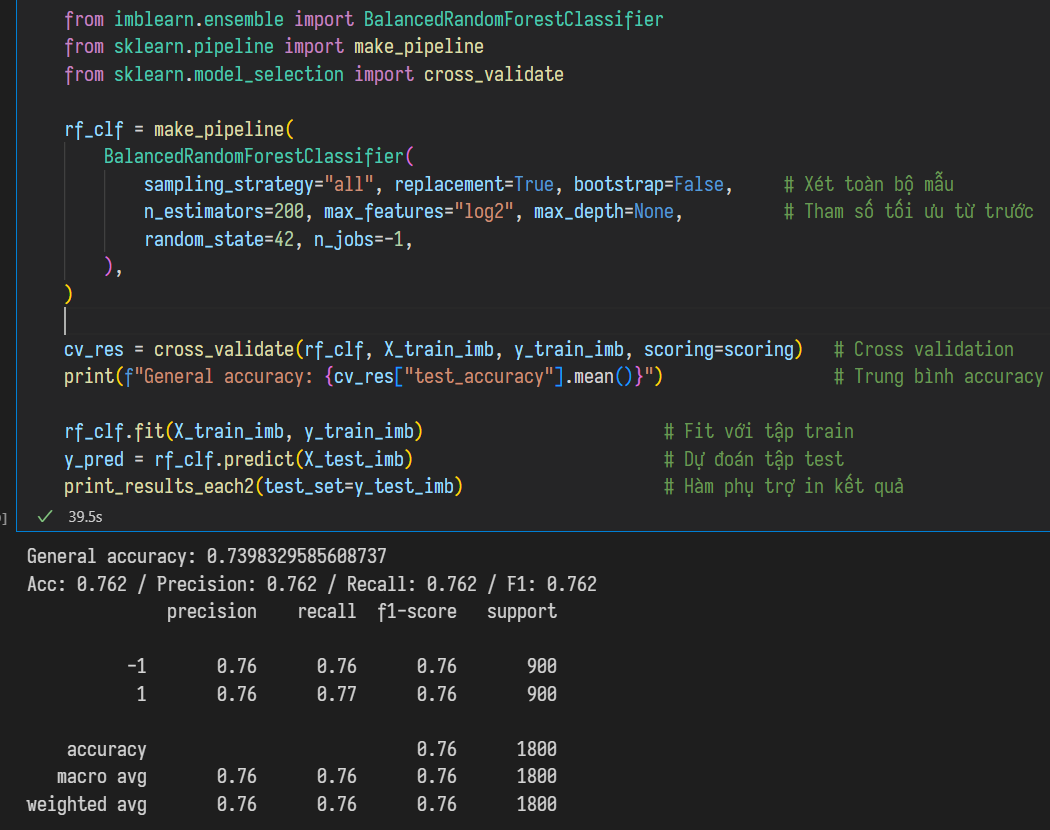
\includegraphics[width=1\textwidth]{images/code-5.16-imblearn1.png}
\end{center}

Ngoài ra, còn có nhiều kỹ thuật khác trong thư viện \texttt{imbalanced-learn} dùng để xử lý dữ liệu mất cân bằng. Ta có thể đặt thêm giả thuyết về dữ liệu hiện tại, và thử nghiệm với nhiều kỹ thuật hơn.

\subsection{Kết luận, hướng phát triển}
Như vậy, ta đã áp dụng nhiều phương pháp để huấn luyện một mô hình học máy thực hiện tác vụ phân tích quan điểm Tiêu cực hoặc Tích cực, và độ chính xác 76.2\% đạt được là tương đối tốt. Có rất nhiều tiềm năng để phát triển mô hình này. Đầu tiên, ta có thể sử dụng các mô hình học máy khác phức tạp hơn, sử dụng Transformer \cite{datta2024transformers}, cơ chế Attention cùng các mô hình Học sâu như mạng Nơ-ron, v.v. Phần hiệu chỉnh thông số có thể thử với nhiều thông số hơn, áp dụng nhiều kỹ thuật trong Xử lý ngôn ngữ tự nhiên hơn.\\

Ngoài ra, ta có thể cải thiện thêm ở phần dữ liệu đầu vào. Trên hết là một Tokenizer để phân tách các từ tiếng Việt tốt hơn, phương pháp vector hóa dữ liệu tốt hơn \cite{Doan_2022}, sau đó là tối ưu hóa danh sách stopword. Ta cũng có thể thử với nhiều phương pháp giảm sự mất cân bằng trong dữ liệu, và cuối cùng, ta cần thêm dữ liệu để có thể dự đoán tốt hơn.